\documentclass[12pt,a4paper]{article}
\usepackage[onehalfspacing]{setspace}

% Packages
\usepackage[utf8]{inputenc}
\usepackage[margin=2.5cm]{geometry}
\usepackage{amsmath, amssymb}
\usepackage{graphicx}
\usepackage{subcaption}
\usepackage{hyperref}
\usepackage{multirow}
\usepackage[table]{xcolor}
\usepackage{tabularx}
\usepackage{hyperref}

\usepackage{tikz}
\usepackage{float}
\usepackage[T1]{fontenc}
\usepackage{upquote}

\usepackage{subcaption} % for subfigures

\usepackage[backend=biber, style=numeric, sorting=none]{biblatex}
\renewcommand*{\multicitedelim}{\addcomma}

% Bibliography file
\addbibresource{references.bib}
\hypersetup{
    colorlinks=true,
    linkcolor=blue,
    citecolor=blue,
    urlcolor=blue
}

\setlength{\parindent}{0pt}   % Remove paragraph indentation
\setlength{\parskip}{1em}     % Add vertical space between paragraphs


\usepackage{pdflscape}  % for landscape pages
\usepackage{geometry}
\usepackage{booktabs}   % nicer tables
\usepackage{adjustbox}  % to scale table if needed

\begin{document}


\begin{titlepage}
 \vspace*{\fill}
    \centering
    {\Huge\bfseries Self-Training with Structured Data for Efficient Insect Pest Detection\par}
    \vspace{1cm}
{\LARGE Bachelor’s Thesis\par}
    \vspace{1cm}
    
    \centering
    {\large
    Christoph Wald\\
    Matrikelnummer 17515905\\
    christoph.wald@stud.uni-goettingen.de\\
    \vspace{1\baselineskip}
    Supervisors: \\
    Prof. Alexander Ecker (Georg-August-Universität Göttingen)\\
    Dr. Elias Böckmann (Julius-Kühn-Institut Braunschweig)\\
    \vspace{1\baselineskip}
    {\today}\\
    }

     \vspace*{\fill}
\end{titlepage}

\newpage

\tableofcontents

{\color{red} Question@Elias: Ich habe am Ende einen Glossar angefangen. Hilft dir das? Wenn ja, soll das ausführlicher oder fehlt was? Wenn nein, kann ich irgendwas anderes tun oder ist das alles so ok für dich mit den ganzen Fachbegriffen?}

\section{Introduction}

Insect pests are responsible for significant production losses in agriculture \cite{climate}. However, pesticides threaten the environment by reducing biodiversity \cite{mamy:hal-03777257}, particularly among insects, including pollinators that support agricultural production \cite{Smith2022PollinatorDeficits}. Overuse of pesticides causes resistance in pests. Additionally, global warming leads to increasing pest populations, which aggravates the problem further \cite{climate}. To address these challenges, the concept of integrated pest management (IPM) was developed. As defined by the Food and Agriculture Organization of the United Nations (FAO), it sets the goal of minimizing the use of pesticides by applying alternative management strategies wherever possible \cite{IPM_FAO, IPM_book}. %For a detailed look into to history and components of IPM compare Messelink and Kruidhof 2019 \cite{IPM_book}. 
IPM is also the legal basis for the use of pesticides in the EU \cite{IPM_EU}, which, among other things, prescribes the monitoring of insect pests when using pesticides. This enables the early and targeted use of pesticides for only small infested patches, the use of less harmful pesticides, or alternative ways of control like beneficial insects. Monitoring is usually based on setting up a grid of sticky traps, which are regularly checked for trapped insects. Because the manual counting requires expertise and takes a lot of time, it is not feasible for larger applications \cite{survey2022}. Hence, computer vision-based systems for automated monitoring of insect pests are considered to be part of the solution. Ongoing efforts to automatize insect pest monitoring have more recently adopted the methods of deep learning (see the surveys Teixeira et al. 2023 \cite{survey2023} and Mittal et al. 2024 \cite{survey2024b}). 
My project aims to facilitate the implementation of deep learning-based, automated insect pest monitoring in the controlled environment of the greenhouse.

The dominant approach in pest monitoring in general involves the supervised training of YOLO models. YOLO ("You Only Look Once") is a deep learning architecture that unifies the tasks of object localization and classification into a single step. It was introduced by Redmon et al. in 2016 \cite{redmon2016you} and has been improved on since then in several iterations by different contributors. For greenhouses, specifically designed neural network models have been employed successfully in 2021 \cite{rustia_automatic_2021, li_field_2021}, but the recent studies from 2023 onwards use YOLO models on individual datasets \cite{costa_intelligent_2023, zhang_automatic_2023, wang_deep-learning-based_2024, shi_small_2025}. These six papers all report high performance, with mean average precision (mAP) or F1 scores ranging from 0.89 to 0.94.

Main challenges in the implementation are the small size of pests—which, even with high-resolution cameras, occupy only a very tiny fraction of an image—and the high degree of morphological variation among individuals. In less controlled environments additional complications arise from high morphological similarity between different species.
These challenges create a demand for large annotated datasets; however, the collection and labeling of biological data require considerable effort and expertise. As a result, datasets are often small and exhibit other limitations, such as class imbalance. For an overview of these specific challenges, see Teixeira et al. (2023) \cite{survey2023}. As a remedy, the authors recommend semi-supervised learning (SSL), a family of methods for training with only partially data. Despite this, no survey reports applications of SSL in the field of pest monitoring in general and only one study in the context of the greenhouse makes use of SSL methods. Rustia et al. \cite{rustia_online_2021} proposed a self-training pipeline as a supplement to a fully supervised model as early as 2021. While the results were promising, the implementation was highly intricate, involving multi-stage setups with hand-tailored solutions. This complexity may explain why the approach has not been further explored. Outside of the greenhouse, in open-field settings, some efforts were made from 2024 onwards, either focusing on a single insect species with more diverse backgrounds or on a set of larger insects \cite{li_mateacher_2024, majewski_improved_2024, zhou_mutual_2024, zhou_perceptive_2025, gomez-zamanillo_semi-supervised_2025}. Another notable paper in this context is Dang et al. (2024) \cite{dang_efficient_2024}, who employ a field dataset of ten larger insect species and perform segmentation without manual annotation by leveraging a grounding language–image model. While extending this approach with classification and adapting it to the smaller insect pests typically found in greenhouses might be feasible, grounding models will not be considered in this study due to their limited speed and efficiency compared to YOLO-based methods. 

Table~\ref{tab:literature-overview} below shows an overview over the relevant literature. Green indicates a correspondence with the demands of my project, red the opposite, and orange overlappings. Because of the differing datasets and metrics, the results are not directly comparable and left out. Also not seen in the table are the pest classes included in the datasets: Only Rustia et. al \cite{rustia_automatic_2021} covered the same pest classes featured in this project. As of now no YOLO model has been trained to identify common greenhouse pests without relying on supervised training. Although working solutions for automatic insect pest monitoring in the greenhouse have been successfully tested, practical deployment stagnates and is hindered by the need for large, manually annotated datasets for new target domains. To my knowledge, there is no adequate method to reduce the amount of labels needed. The goal of the thesis is therefore an improvement in implementation efficiency by adapting the labeling and training method.

\newpage

\begin{table}[htbp]
\centering
{\footnotesize
\begin{tabularx}{\textwidth}{l c c c l}
\hline
\textbf{Authors (Year)} & \textbf{Greenhouse} & \textbf{YOLO} & \textbf{Training}  \\
\hline

Li et al. 2021 \cite{li_field_2021}
& \cellcolor{green!40}yes & \cellcolor{red!40}no & \cellcolor{red!40} supervised \\

Rustia et al. 2021 \cite{rustia_automatic_2021}
& \cellcolor{green!40}yes & \cellcolor{red!40}no & \cellcolor{red!40} supervised \\

Rustia et al. 2021 \cite{rustia_online_2021}
& \cellcolor{green!40}yes & \cellcolor{red!40}no & \cellcolor{orange!40} SSL (predicted pseudo-labels by separate pipeline)\\

Costa et al. 2021 \cite{costa_intelligent_2023}
& \cellcolor{green!40}yes & \cellcolor{green!40}yes & \cellcolor{red!40} supervised \\

Zhang et al. 2023 \cite{zhang_automatic_2023} 
& \cellcolor{green!40}yes & \cellcolor{green!40}yes & \cellcolor{red!40} supervised \\

Li et al. 2024 \cite{li_mateacher_2024}
& \cellcolor{red!40}no & \cellcolor{red!40}no & \cellcolor{orange!40} SSL (teacher-student) \\

Majewski et al. 2024 \cite{majewski_improved_2024}
& \cellcolor{red!40}no & \cellcolor{green!40}yes & \cellcolor{orange!40} SSL (pseudo-labels) \\

Wang et al. 2024 \cite{wang_deep-learning-based_2024}
& \cellcolor{green!40}yes & \cellcolor{green!40}yes & \cellcolor{red!40} supervised \\

Zhou et al. 2024 \cite{zhou_mutual_2024}
& \cellcolor{red!40}no & \cellcolor{red!40}no & \cellcolor{orange!40} SSL(teacher-student ) \\

Gomez-Zamanillo et al. 2025  \cite{gomez-zamanillo_semi-supervised_2025}
& \cellcolor{red!40}no & \cellcolor{red!40}no & \cellcolor{orange!40} supervised, labels enhanced by image processing \\

Shi et al. 2025 \cite{shi_small_2025}
& \cellcolor{green!40}yes & \cellcolor{green!40}yes & \cellcolor{red!40} supervised \\

Zhou and Shi 2025 \cite{zhou_perceptive_2025} 
& \cellcolor{green!40}yes & \cellcolor{red!40}no & \cellcolor{orange!40} SSL(teacher-student ) \\

\hline
\end{tabularx}
}
\caption{Overview over relevant papers.}
\label{tab:literature-overview}
\end{table}

 I propose that given a specifically structured training dataset, a model can be trained without the need for manual labeling. This is achieved by a combination of image processing and a semi-supervised learning method (SSL) called self-training. The results are expected to contribute to a software foundation for a low-cost, open-source insect pest monitoring solution. It should be trainable on a single GPU and also provide efficient inference. Such a system could support practical deployment in greenhouse production settings and serve as a research tool for further studies.
 
 The key requirement for the proposed solution is the specific structure of the dataset, which should be partitioned into subsets. All images in one subset should only contain one specific pest class as objects. With already existing labels a supervised YOLO model is trained as reference point, which should reach achieve at least 0.9 precision and 0.8 recall per class. Precision is prioritized in this target values over recall for two reasons. First, recall can be improved later through denser placement of sticky traps, whereas precision depends primarily on model quality. Second, low precision risks erroneous pesticide use, which conflicts with the principles of IPM. 
 
The envisioned adapted automated labeling and SSL is done in two stages. First, with image processing segmentation algorithms bounding boxes for the pest classes are created. Since the images are presorted to contain only one pest class, the detected bounding boxes can be directly associated with the corresponding label, yielding a partially labeled dataset. In the second stage, the partially labeled dataset as given by stage one is used in a self-training SSL framework with an adapted YOLO to produce a model.

{\color{red} ToDo: Actualize this in the end, especially the final solution found for the thrips problem}

\section {Methods}

\subsection{Data}

\subsubsection{Dataset description}
\label{sec:data_description}
{\color{red} ToDo: Include mixed images, also in the other sections}\\
The data is provided by the Julius-Kühn-Institut (JKI) and was collected as part of the Smart-Checkpots project \cite{raaz_smart_2023}. It consists of four subsets of images each associated with one of four insect pest classes (see Table 2). Every image in a subset is supposed to depict several instances of only one pest class  trapped on a yellow sticky trap (YST)\footnote{In general, there are different types of traps e.g. pheromone traps and there are also sticky traps with different colours, but YSTs are the most commonly used traps in greenhouses. Yellow is a compromise which most attract most insect pests.} (see Figure~\ref{fig:example_YSTs}). 

\begin{table}[h!]
\centering
\begin{tabular}{|l|p{6cm}|l|}
\hline
\textbf{Common Name} & \textbf{Scientific Name} & \textbf{EPPO Code} \\ \hline
Fungus gnats & Bradysia impatiens, \textsc{Johannsen} 1912 (Diptera: Sciaroidea) & BRAIIM \\ \hline
Tomato leaf miner & Liriomyza bryoniae, \textsc{Kaltenbach} 1858 (Diptera: Agromyzidae) & LIRIBO \\ \hline
Western flower thrips & Frankliniella occidentalis, \textsc{Pergande} 1895 (Thysanoptera: Thripidae) & FRANOC \\ \hline
Greenhouse whitefly & Trialeurodes vaporariorum, \textsc{Westwood} 1856 (Hemiptera: Aleyrodidae) & TRIAVA \\ \hline
\end{tabular}
\caption{Overview of insect pest classes.}
\label{tab:insect_classes}
\end{table}

\begin{figure}[H]  % 
    \centering
    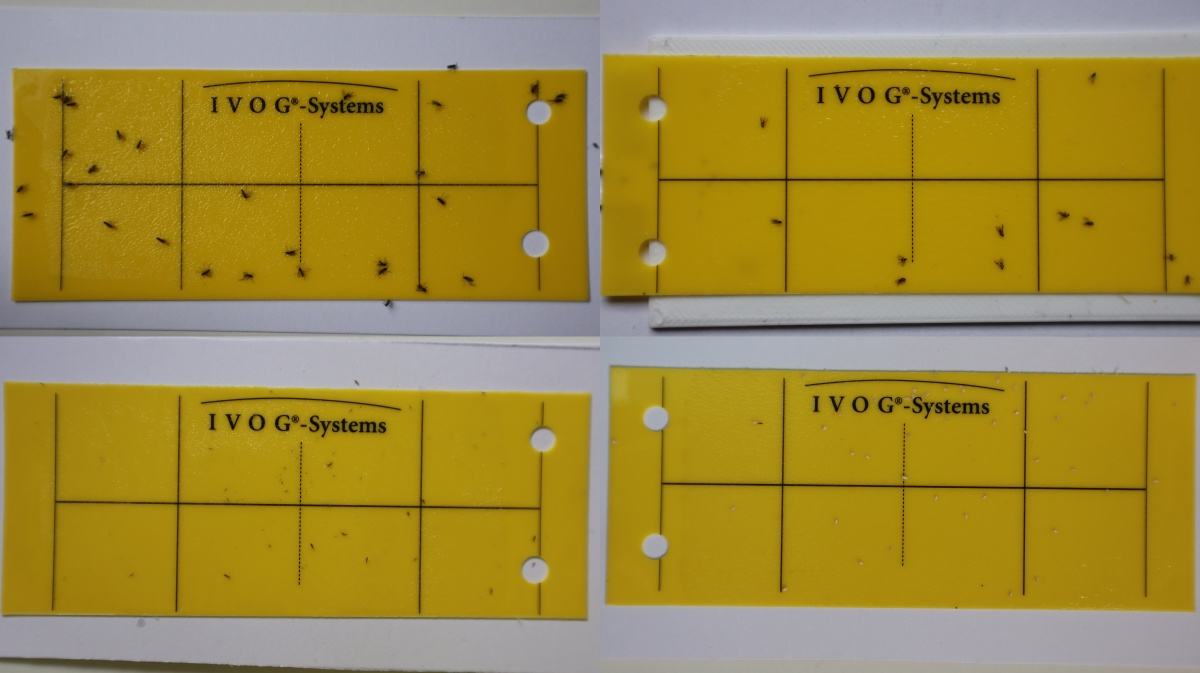
\includegraphics[width=1.0\textwidth]{images/figure1.jpg}  % Adjust width as needed
    \caption{Example images from the four subsets with images from fungus gnats, leaf miner flies, thrips, and whiteflies (left to right, top to bottom). Reduced resolution.}
    \label{fig:example_YSTs}
\end{figure}


The chosen insect pests are common in greenhouses, particularly on crops such as tomatoes and cucumbers, where they can cause severe damage, up to complete crop loss \cite{rustia_automatic_2021}. As Figure~\ref{fig:example_insects} shows, the size of the pest classes and thereby the number of pixels they cover differs considerable. In thrips, also male and female differ in appearance. The female individuals are larger and have good contrast against the yellow background, whereas the smaller and more transparent males are harder to detect (Row 3, box 3,7, and 9). \\
{\color{red} Question@JKI: Are there wrong insects in the figure? Are male/female thrips assigned correctly?}

\begin{figure}[H]  % 
    \centering
    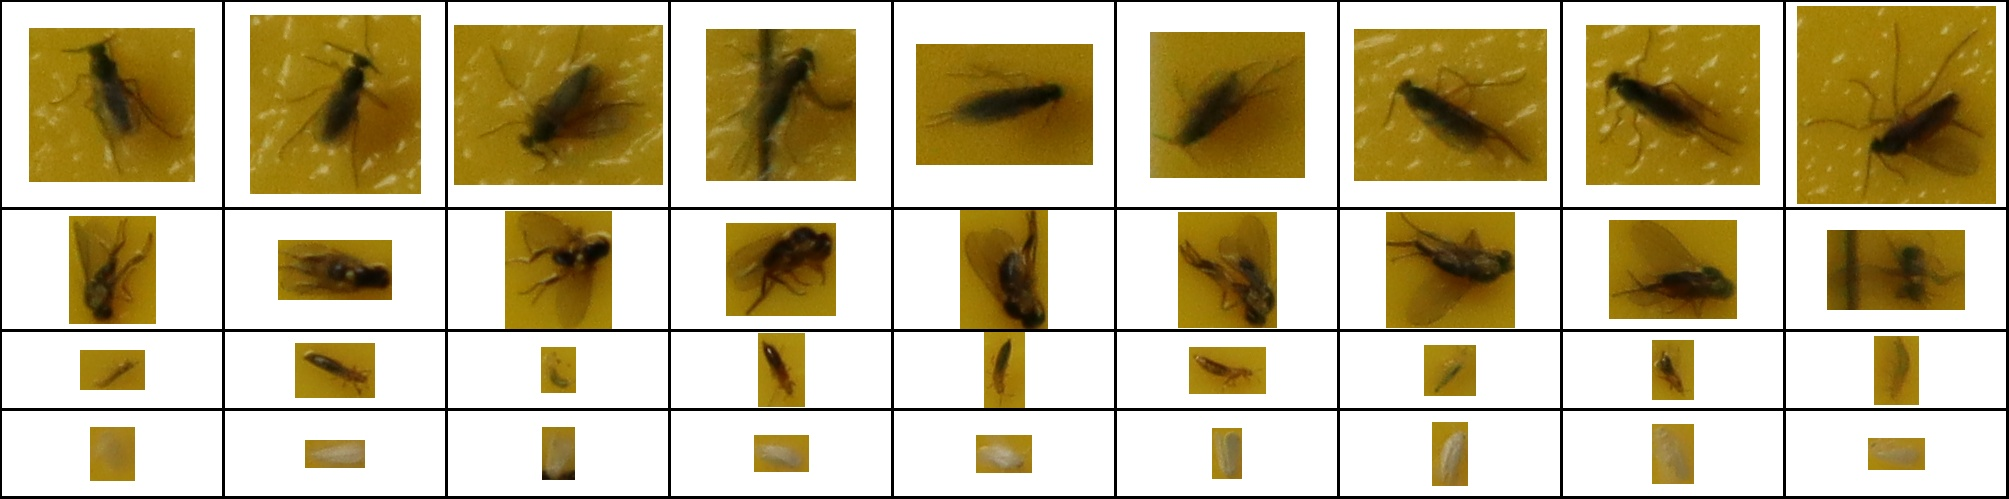
\includegraphics[width=1.0\textwidth]{images/figure2.jpg}  % Adjust width as needed
    \caption{Cropped boxes with fungus gnats, leaf miner flies, thrips, and whiteflies (top to bottom). Original resolution.}
    \label{fig:example_insects}
\end{figure}

The populated YSTs in this dataset were created at the JKI by breeding the insects to the adult stage in a closed environment (see Figure~\ref{fig:breeding}) and exposing the YST in the environment for some time until it became populated. The traps were then immediately attached onto a piece of white paper, and pictures were taken with a Canon EOS M50 Mark II on a tripod at a distance of approximately 13 cm (see Figure~\ref{fig:canon}) and a resolution of 6000 × 3368 pixels, resulting in files of about 5–7 MB. No artificial light was used to avoid reflections. The pictures have slightly different view angles and different lighting conditions, some still affected from reflections and some having areas with low sharpness. Some of these aspects may be also be part of the real data to be processed after training.

\begin{figure}[H]
    \centering
    % First image
    \begin{subfigure}{0.45\textwidth}
        \centering
        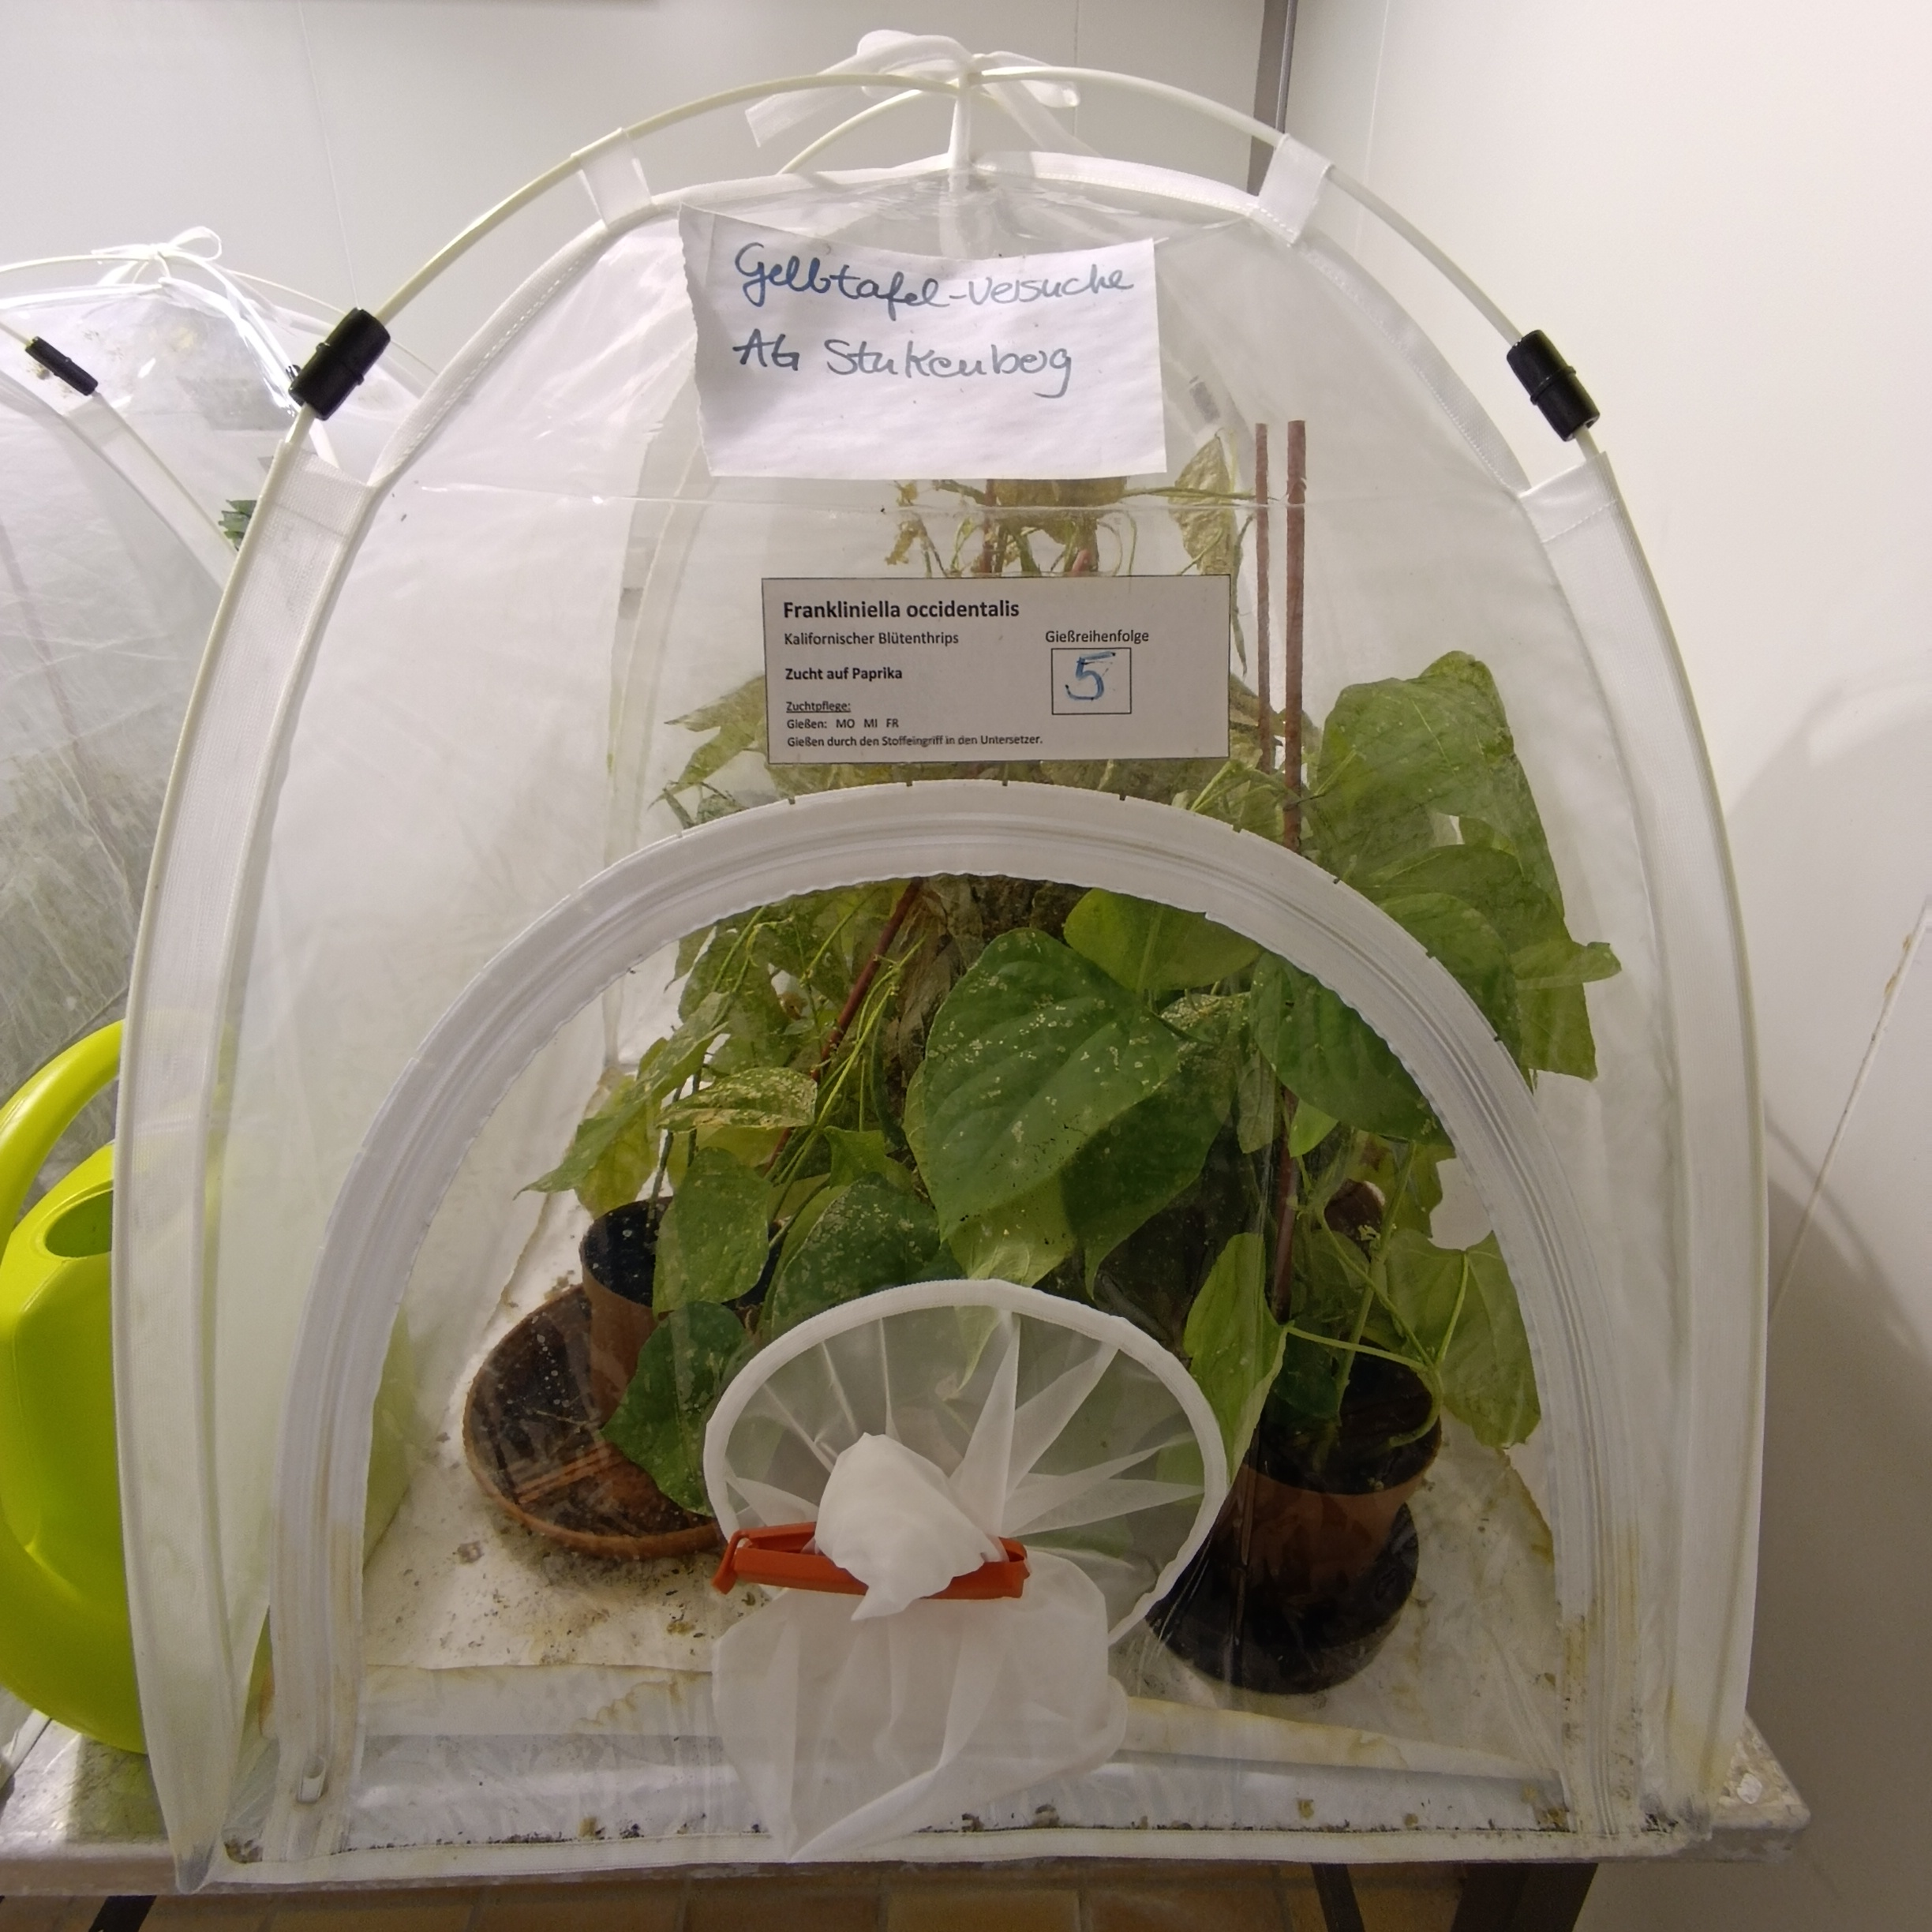
\includegraphics[width=\linewidth]{images/figure3a_zucht.jpg}
        \caption{Breeding station}
        \label{fig:breeding}
    \end{subfigure}
    \hfill
    % Second image
    \begin{subfigure}{0.45\textwidth}
        \centering
        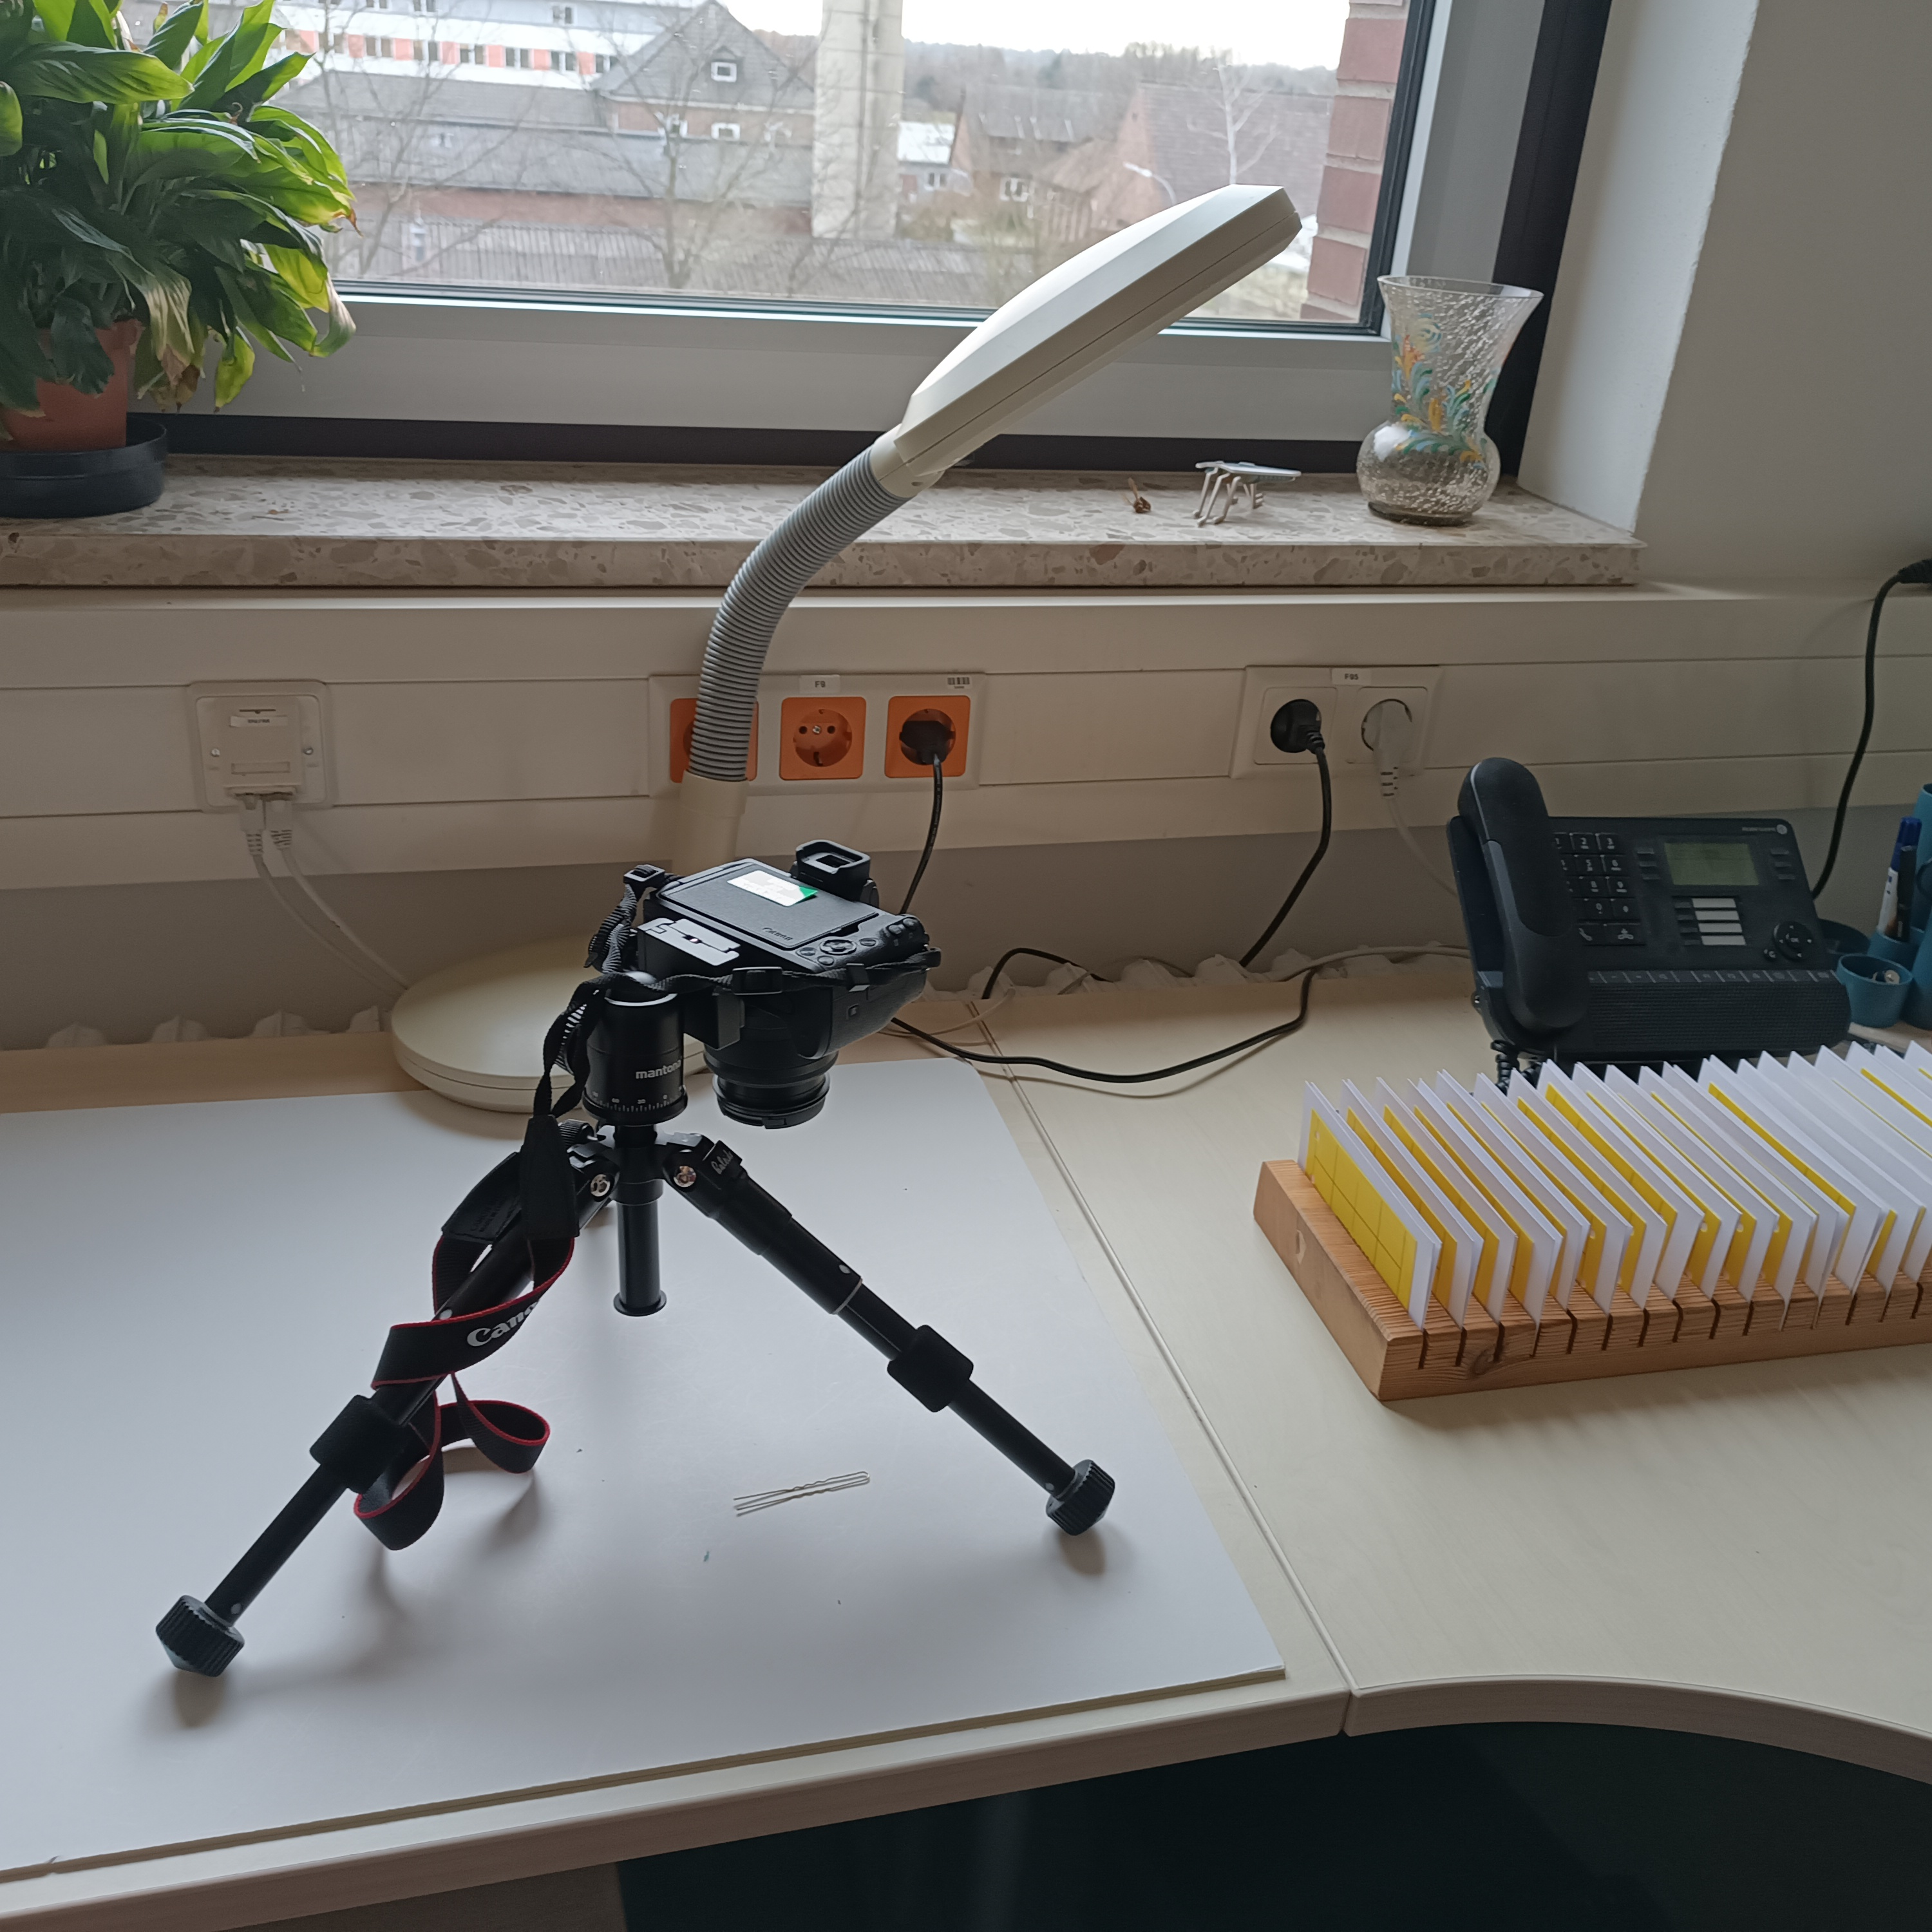
\includegraphics[width=\linewidth]{images/figure3b_canon.jpg}
        \caption{Camera setup}
        \label{fig:canon}
    \end{subfigure}
    
    \caption{Data creation, pictures with kind permission M. Pollmann, JKI}
    \label{fig:data_creation}
\end{figure}

{\color{red} Question@JKI: How was this done exactly and why?}\\
{\color{red} Question@JKI: Is Figure 4b an example for not labeled male thrips or just some larvae present?}\\
{\color{red} ToDo: Describe thrips image creation and the problems it presents and rewrite the following paragraph}\\
On the images of the thrips subset sometimes larger amounts of foliage (see Figure~\ref{fig:folliage}) are present. Also there are thrips in larval stages, which are hard to distinguish from the male individuals. This posed difficulties for the manual labeling, but is also a critical problem for the automated labeling process.

\begin{figure}[H]
    \centering
    % First image
    \begin{subfigure}{0.45\textwidth}
        \centering
        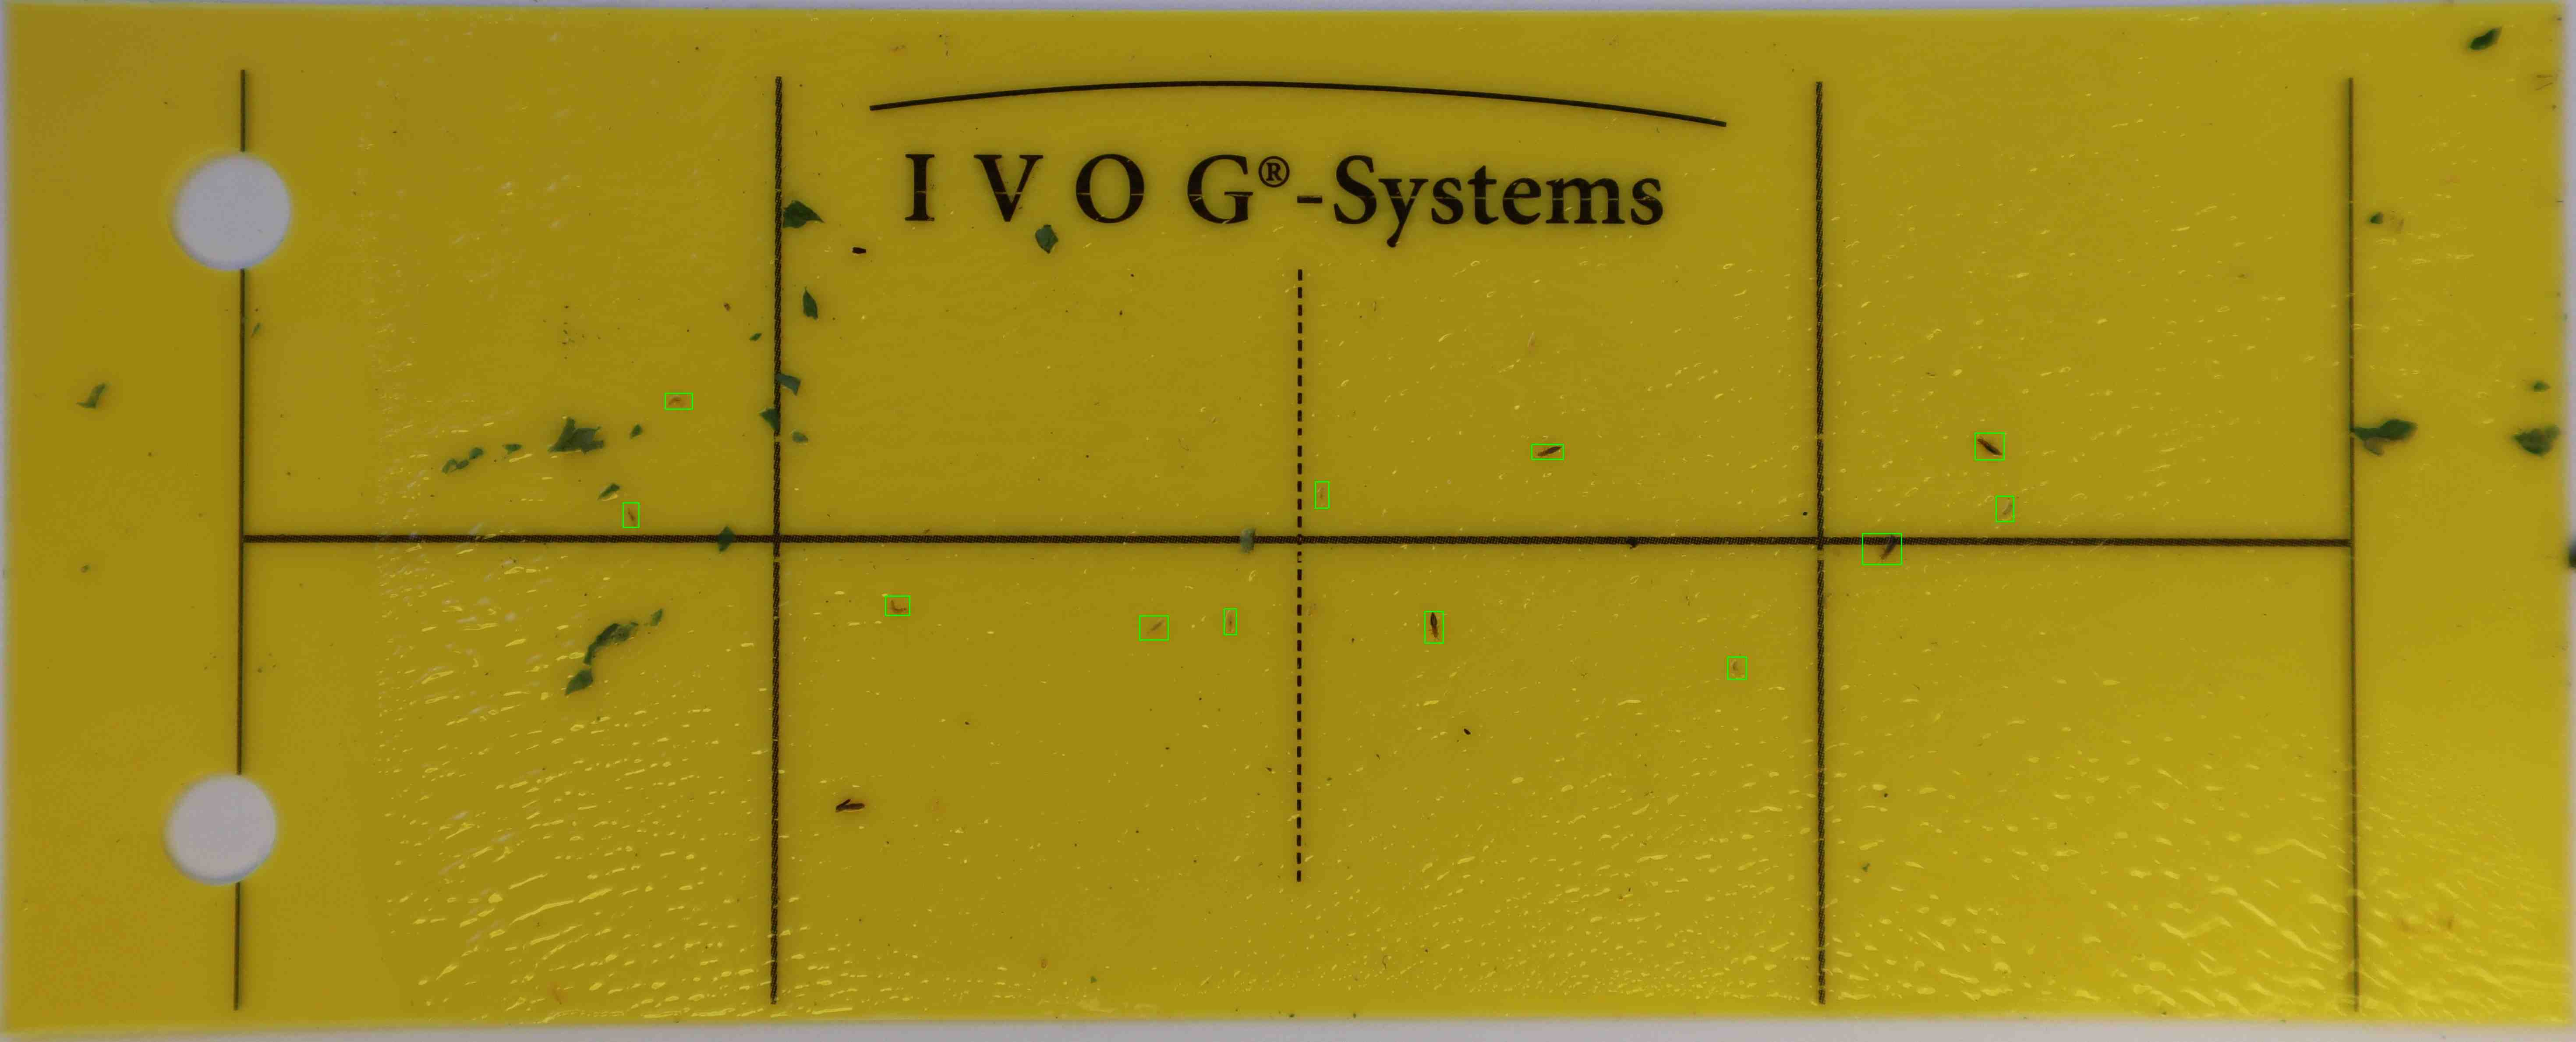
\includegraphics[width=\linewidth]{images/figure_folliage_FRANOC_0046_with_boxes.jpg}
        \caption{Labeled thrips with foliage on the image}
        \label{fig:folliage}
    \end{subfigure}
    \hfill
    % Second image
    \begin{subfigure}{0.45\textwidth}
        \centering
        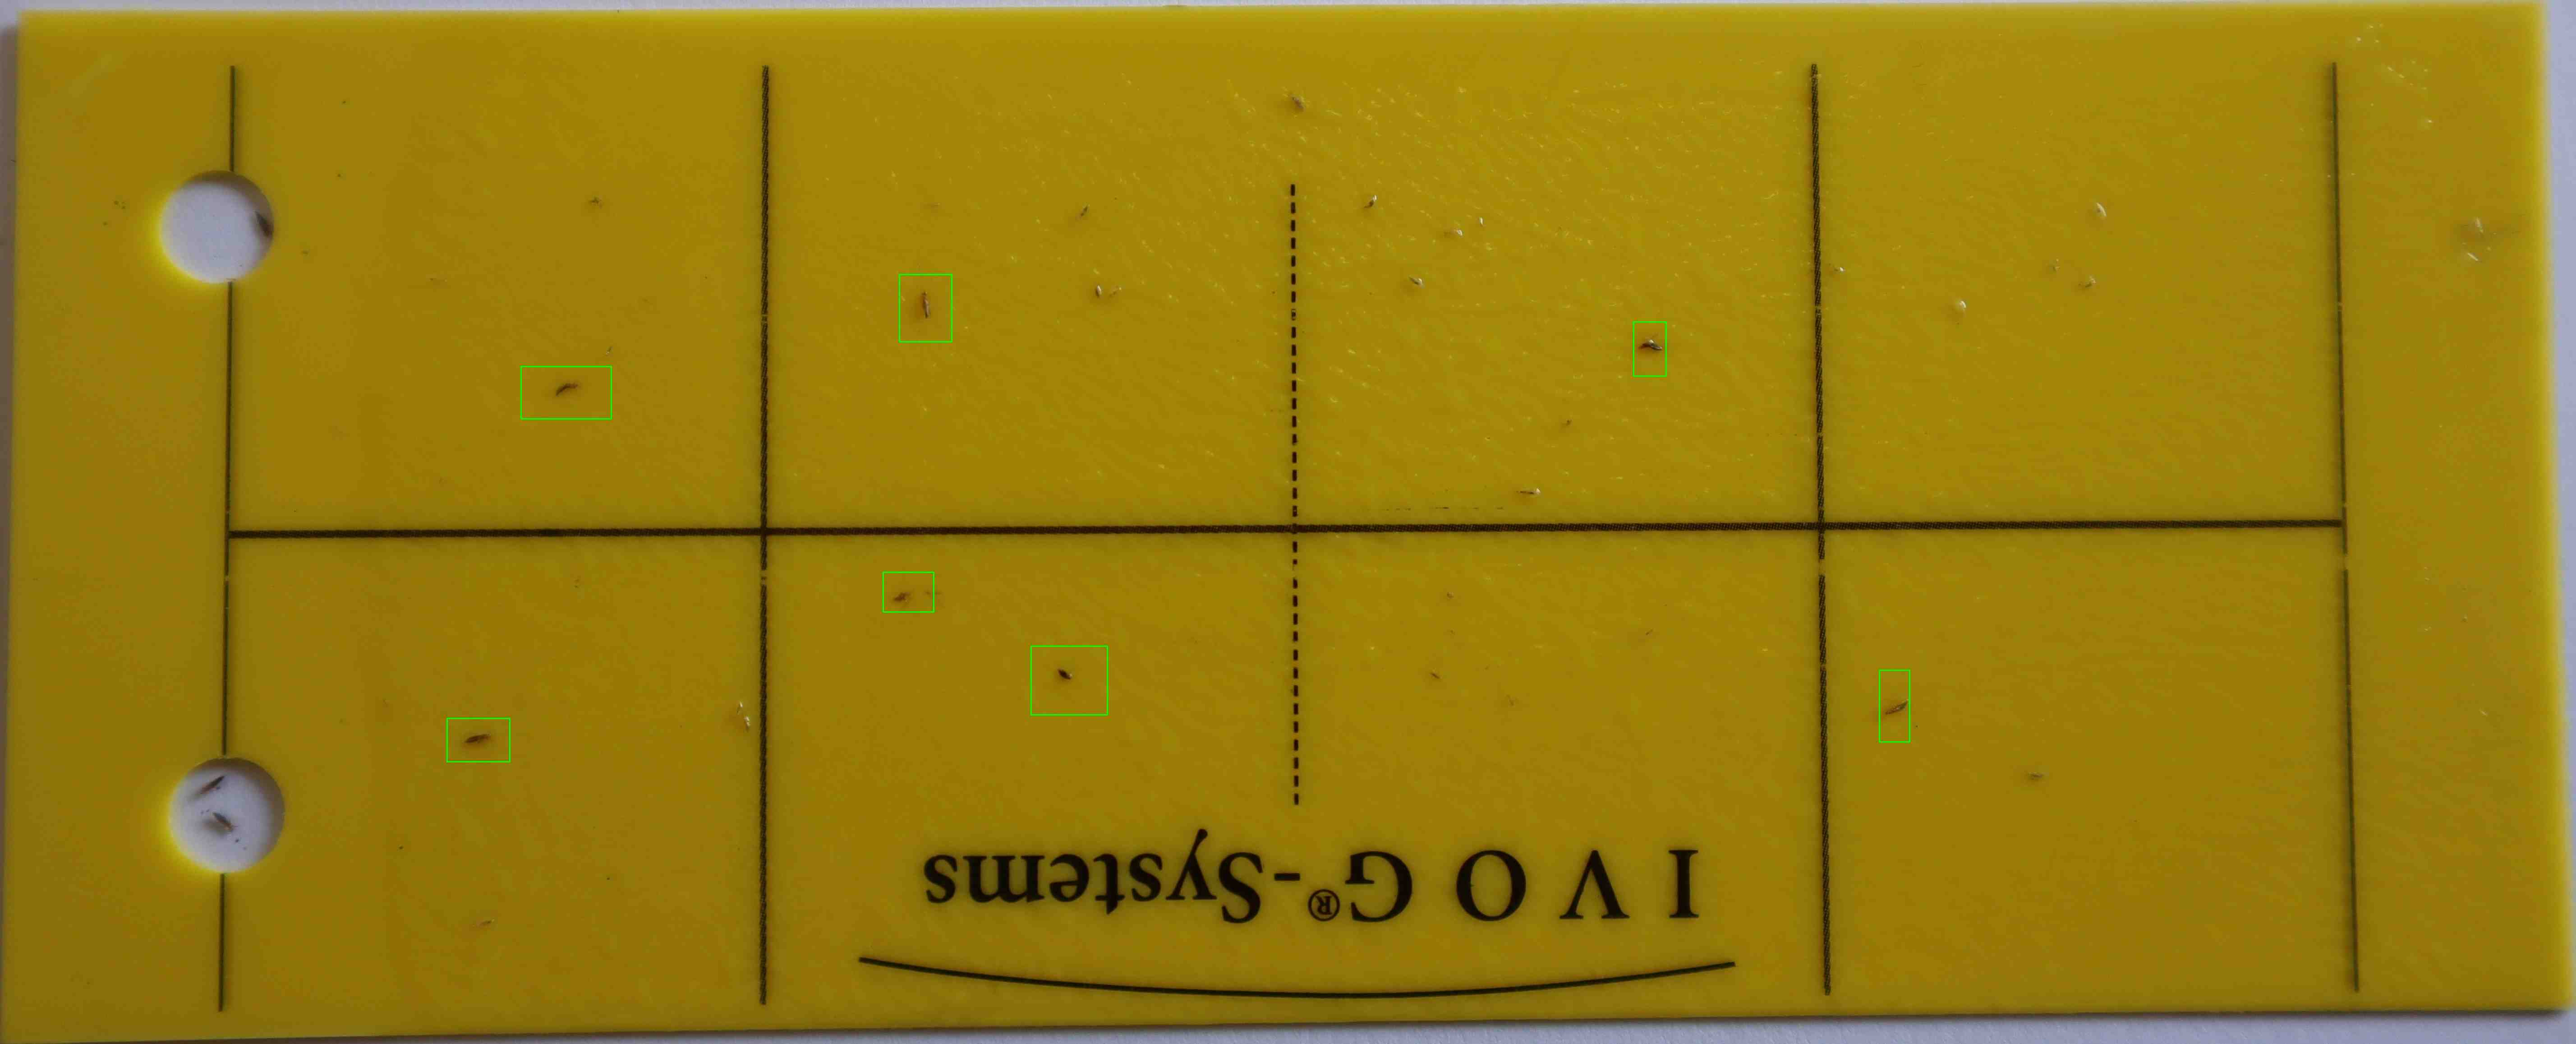
\includegraphics[width=\linewidth]{images/figure_large_boxes_FRANOC_0675_with_boxes.jpg}
        \caption{Labeled thrips with large bounding boxes}
        \label{fig:large_boxes}
    \end{subfigure}
    
    \caption{Examples for thrips images and labels}
    \label{fig:thrips_YSTs}
\end{figure}

For each pest class a proportion of images were manually labeled. Other than for the thrips, visual inspection showed the label quality to be consistent, although with a noticeable proportion unlabeled individuals for the fungus gnats. Also the size of the bounding boxes may differ for the batches that different persons labeled (see Figure~\ref{fig:thrips_YSTs}), which will be taken into account. 

\subsubsection{Preprocessing}

As preparation for the project, I sorted the image files by their creation time given by the metadata. The first 100 images for each class were visually inspected and images with identical YSTs and different camera settings were removed manually. These were leftovers of early experiments with the camera setup. I removed further duplicates (identical images)  by comparing file checksums. Images with labels that indicated no insects or unexpected insects not belonging to the class of the subset were also removed. 

For the thrips, an additional visual inspection on this subset was carried out. This led to the exclusion of 200 images with wrong labels or too much other objects. To improve the quality of the thrips labels further, for the remaining pictures the bounding boxes given by the labels were cut out and inspected by an expert from the JKI. 1276 labels were identified as incorrect and removed from the label files.

Table~\ref{tab:insect-stats} shows the number of images and labels after all cleaning reported in this section. The dataset is imbalanced, both in terms of the number of labeled images per class and the mean number of instances per image.
%00d plot statistics

\begin{table}[htbp]
\centering
\begin{tabular}{lrrrrrr}
\hline
Class & Images & Labeled & \begin{tabular}[c]{@{}c@{}}Fraction \\ labeled\end{tabular} & \begin{tabular}[c]{@{}c@{}}Instances \\ labeled\end{tabular} & \begin{tabular}[c]{@{}c@{}}Mean instances \\ per image\end{tabular} \\
\hline
FungusGnats     & 1328 & 1018 & 76.66 \% & 33373  & 32.78  \\
LeafMinerFlies  & 1422 & 659  & 46.34 \% &  6518  &  9.89  \\
Thrips          & 1134 & 392  & 34.57 \% &  5453  & 13.91  \\
WhiteFlies      & 1105 & 433  & 39.19 \% & 25735  & 59.43  \\
\textbf{Total}  & \textbf{4989} & \textbf{2502} & \textbf{50.15 \%} & \textbf{71527}  & \textbf{28.59} \\

\hline
\end{tabular}
\caption{Annotation statistics after cleaning and preprocesing.}
\label{tab:insect-stats}
\end{table}

Because of the summed difficulties the thrips images and labels posed, the class had to be discarded for further experiments after the supervised training, which showed that no satisfying results are to be expected in the proposed self-training. There are three major reasons for this decision: low sample size, presence of non-target objects, and low label quality.  Because of size and morphological differences between adult males and females the thrips is the hardest pest class to detect and has to be represented with an according number of images and instances in the dataset. Unfortunately, after cleaning the thrips subset has the lowest number of images and labels in the dataset. Furthermore the thrips are easiest to be mixed up with other objects like foliage and therefore require clean images. But the thrips images are the only pest class that has lots of non-target objects, including thrips larvae on their images. The 1276 false labels clearly show that the automated labeling cannot work under the assumption that all objects on an image are instances of the respective pest classes. Finally, the inconsistent labeling quality prohibits proper testing. 

Some labels were found to contain negative coordinates. After visual inspection of samples, these values were interpreted as their absolute counterparts, since this matched the actual object positions. The underlying cause of the negative coordinates could not be identified.

\subsubsection{Splitting}

From the dataset, three sets are built (see Figure~\ref{fig:split}). 

\begin{figure}[H]
    \centering
    % First image
    \begin{subfigure}{0.45\textwidth}
        \centering
        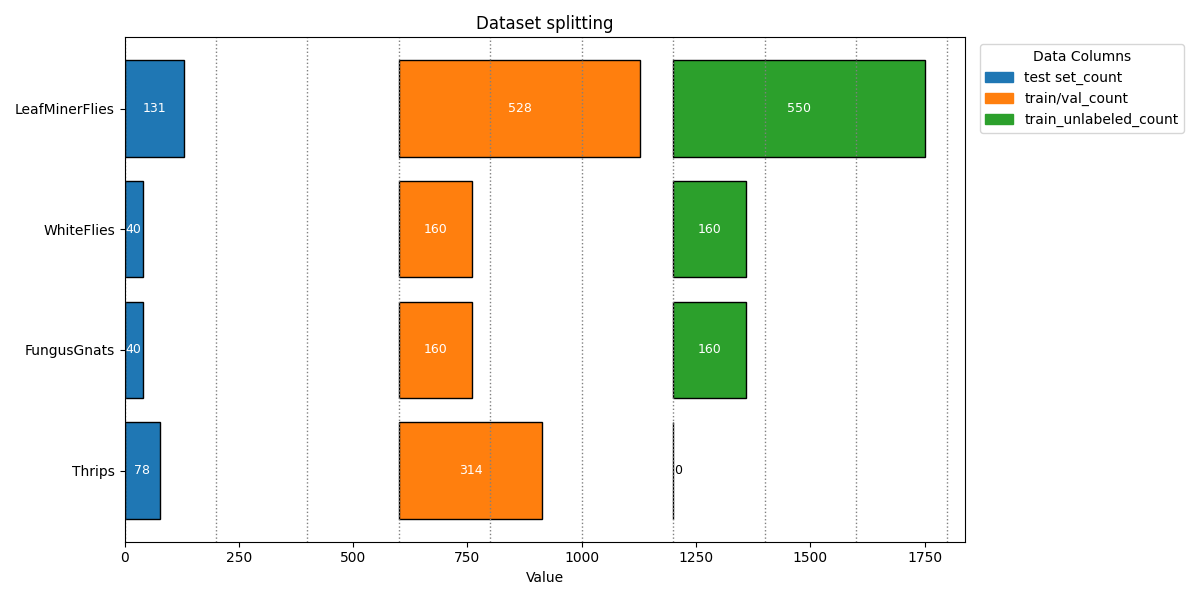
\includegraphics[width=\linewidth]{images/dataset_splitting.png}
        \caption{Subsets}
        \label{fig:split}
    \end{subfigure}
    \hfill
    % Second image
    \begin{subfigure}{0.45\textwidth}
        \centering
        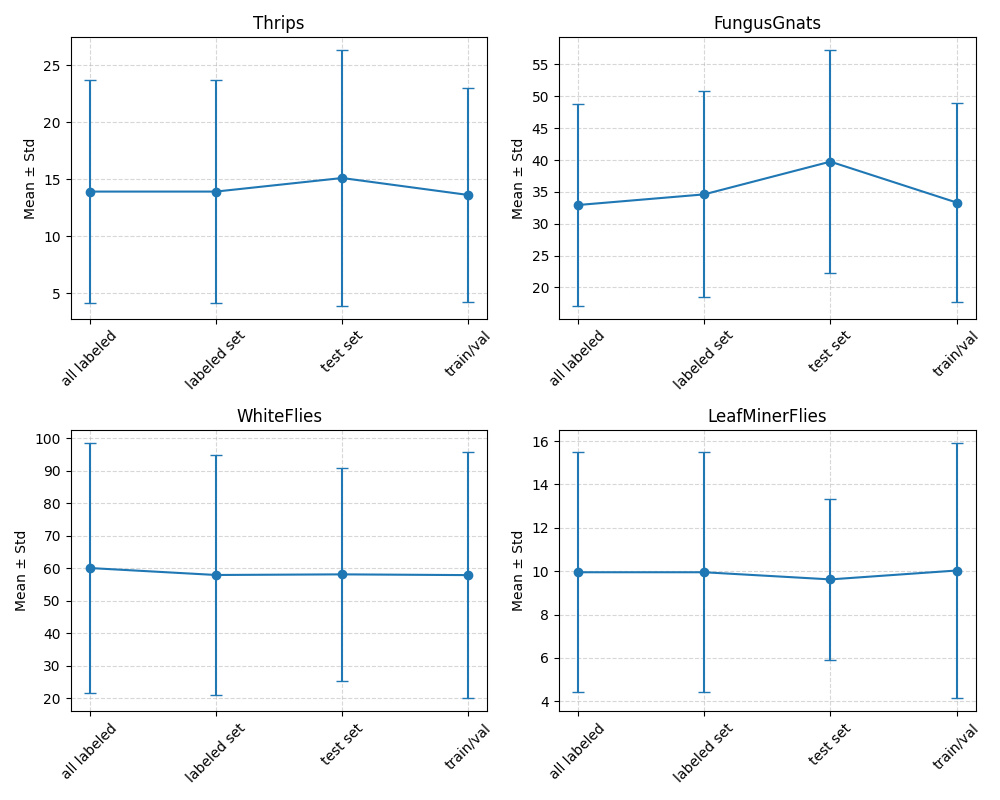
\includegraphics[width=\linewidth]{images/labeled_sets.png}
        \caption{Mean instances per image for the labeled (sub)sets}
        \label{fig:mean_labels}
    \end{subfigure}
    
    \caption{Data splitting}
    \label{fig:dataset_splitting}
\end{figure}

To balance the labeled sets, only 200 randomly chosen labeled images from the fungus gnat and the white flies are used, because these pest classes have considerably more instances on a single image than thrips and leaf miner flies. The other labels are discarded and the images retained as unlabeled. The labeled set is then further divided randomly into 20\% test set and 80\% training set. As Figure~\ref{fig:mean_labels} shows, the mean instances per image are comparable for the full labeled set, the reduced labeled set, the test set, and the training set. From the unlabeled images excluding the thrips a set is drawn with comparable sizes as the training set. Finally, both training sets are further split into training and validation subsets, using the same 80/20 ratio.

\subsection{Supervised training}

{\color{red} Question@Alex: Do I have to include more info on YOLOv8 here?}\\
{\color{red} Question@Alex: I did not do this by the book. Do I have to redo it?}\\
{\color{red} Question@Alex maybe just train on full images, as escarda did?}\\
{\color{red} Question@Alex Isn't it strange to train on the tiles but predict on the images, because validation test metrics could diverge?}\\
As a reference point for the automated labeling process, a YOLOv8 model is trained using the manual labels provided. The aim is to demonstrate that the data is sufficient to reach the target metrics of a minimum per-class precision of 0.9 and recall of 0.8. Since supervised training is not the main focus of this project, experiments are not designed to fully optimize results. A small YOLOv8s model pretrained on COCO is chosen because initial tests showed that larger models or later versions did not improve performance. With 4-5 GB of weights, the small model also meets the requirement of single-GPU training and the more modular code of version 8 is easier to adapt for self-training. No task-specific pretrained models are available to my knowledge. 

The images are cropped to the size of the YST with color threshold based segmentation (compare YSTs in Figure~\ref{fig:example_YSTs} and Figure~\ref{fig:thrips_YSTs}). This decreases the size of the dataset by 17,1 GB but also introduces different image sizes. Labels are therefore recalculated after cropping. Since YOLO labels are relative to image width and height, the new image dimensions must be used when transforming labels back into absolute coordinates. 

YOLO expects images of size 640x640 and resizes images with larger resolution. Because the insect pest classes are of small size, this resizing might may cause difficulties. Therefore images are tiled. After padding each image such that its dimensions are divisible by 640, the images are tiled into 640×640 patches with a stride of 440. The overlap of 200 pixels corresponds to the size of the largest pest class, the fungus gnats, such that an instance is at least contained in one tile. The labels are recalculated according to the tiles and labels and are only kept if they are contained to at least 80\% inside the respective tile.  The resulting tiles contain a large number of empty background tiles, which account for over 68\% of the tiles in the labeled training set.

{\color{red} Question@Alex: Do I have to document all this augmenation techniques?}\\
Starting from the default settings, short training runs with selected parameter changes were conducted to identify optimization potential, where augmentation settings and the ratio of background to foreground images are identified as the main factors influencing performance. Changing the default optimizer (stochastic gradient descent), learning rate schedule, and loss weights did not yield improvements. Two augmentation parameter sets (see Table~\ref{tab:paramters-supervised}) are tested in longer training runs. Because the dataset already contains considerable variance (see Section~\ref{sec:data_description}), augmentations are applied only subtly. In parameter set 1, the scaling factor is reduced to avoid unrealistic size differences between objects, and the probability of mosaic augmentation is lowered to prevent the model from learning lighting differences between images. A small amount of mixup is introduced with a 5\% probability. All other parameters are kept at the default values. Parameter set 2 is designed to counteract the reduced variance caused by lowering the number of background images in the training set. It retains the changes of Set 1 but additionally reduces the probability of horizontal flipping, to avoid generating mirrored text in the backgrounds. To compensate for the reduced background variance, cropping with a maximum fraction of 10\% is allowed, and multiscale training (rescaling of complete batches) is enabled.

\begin{table}[h]
\centering
\begin{tabular}{lccc}
\hline
\textbf{Parameter} & \textbf{Default} & \textbf{Parameter Set 1} & \textbf{Parameter Set 2} \\
\hline
Scale           & 0.5   & 0.3   & 0.3 \\
Mosaic          & 1.0   & 0.25  & 0.25 \\
Mixup           & 0.0   & 0.05  & 0.05 \\
Crop fraction   & 0.0   & 0.0    & 0.1 \\
Multiscale      & no    & no    & yes \\
FlipLR          & 0.5   & 0.5   & 0.3 \\
\hline
\end{tabular}
\caption{Adapted parameter sets}
\label{tab:paramters-supervised}
\end{table}

For the training runs the proportion of background tiles (tiles without objects) is varied (seeTable~\ref{tab:train_params}). The initial training contains 68\% background tiles, which is reduced to 10\% and 30\% in a number of training runs. To test the effect of the thrips images on the training of the other classes, the set with only 30\% background images is stripped from all images from the thrips subset which changed the background to foreground ratio to 47\%. All but the last three trainings are run 100 epochs and a batch size of 16. Though not necessary for regularization, early stopping with patience 10 is used, to prohibit unneccessary training. Two additional trainings are run with 200 epochs and early stopping and a last one also at 200 epochs without early stopping.

\begin{table}[h!]
\centering
\begin{tabular}{lcccc}
\hline
\textbf{Train} & \textbf{Parameterset} & \textbf{Background} & \textbf{Epochs} & \textbf{Patience} \\
\hline
train1 & 1 & 68 & 100 & 10 \\
train2 & 1 & 10 & 98 & 10 \\
train3 & 2 & 10 & 100 & 10 \\
train6 & 2 & 30 & 100 & 10 \\
train7 & 1 & 30 & 100 & 10 \\
train8 & 1 & 30 & 148 & 10 \\
train9 & 1 & 47* & 111 & 10 \\
train10 & 1 & 47* & 200 & - \\
\hline
\multicolumn{5}{l}{\footnotesize{* 30\% background → thrips deleted}}
\end{tabular}
\caption{Training parameters for different runs.}
\label{tab:train_params}
\end{table}

\subsection{Testing the model}



The prediction on the test set images is done by sliding over full images with a given stride, predicting on the tiles and afterwards filtering the detected bounding boxes. For stride the value used in tiling the training set is compared to a slightly reduced one. Bounding boxes detected are then first filtered by a confidence threshold. As starting point, the confidence threshold chosen during YOLO training (based on the best F1-score across classes) is used. This value gives the optimal balance between precision and recall. Since precision is favored over recall in this study, prediction with confidence values increased by 0.1 and 0.2 are used for testing. Table~\ref{tab:eval_param} ) shows different combination of stride and confidence threshold that are used in testing.

\begin{table}[h!]
\centering
\begin{tabular}{|c|c|c|}
\hline
 & confidence threshold & stride \\
\hline
eval1 & F1max & 440 \\
eval2 & F1max+.1 & 440 \\
eval3 & F1max+.1 & 420 \\
eval4 & F1max+.2 & 420 \\
eval5 & F1max+.2 & 440 \\
\hline
\end{tabular}
\caption{Evaluation settings for F1 and stride values.}
\label{tab:eval_param}
\end{table}

{\color{red} Question: Is the following correctly part of the methods or does it belong to results already?}

Non-maximum suppression (NMS) is used to filter overlapping bounding boxes for the same object. It relies on the intersection of union (IoU) metric, which is the ratio between the area where two boxes overlap and the area that the boxes cover when combined. When two boxes have an IoU above a threshold, only the box with the higher confidence is kept. However, if a small box is completely or partially inside a larger box, the IoU will be low, because the intersection is only as small as the small box and the union is as big as the large box. As visual inspection shows, the small objects in the dataset make it necessary to include an extra filtering for this case. IoU for NMS was set to 0.4 and the threshold to filter out the other case was set to 0.5. See Figure~\ref{fig:iou_problems} a and b for false positives that occour without the extra filter and see Table~\ref{tab:extra_overlap_filtering} that the extra filter reduces the number of false positives.

Comparison to the ground truth also relies on IoU and as usual, predicted bounding boxes were counted as true positives with an IoU equal or larger than 0.5. Again, visual inspection shows small correct predictions inside larger ground truth boxes are not covered by this procedure. In an additional routine, also predicted boxes contained at least with 0.9 of their area in ground truth boxes are counted as true positive. See Figure~\ref{fig:iou_problems} c and d for false positives that occur without the extra comparision and see Table~\ref{tab:extra_overlap_filtering} that the extra comparision reduces the number of false negatives.

\begin{table}[h!]
    \centering
    \begin{tabular}{lccc}
        \toprule
        & TP & FP & FN \\
        \midrule
        No extras & 5646  & 1157 &  993 \\
        Additional containment filtering for NMS & 5644  & 983 & 994  \\
        Additional containment comparison of ground truth & 5788 & 1175 & 850   \\
        Both & 5788 & 839  & 850 \\
        \bottomrule
    \end{tabular}
    \caption{Comparison of detection results under different settings of extra thresholds. Model is taken from training run 7, evaluation setting are set 3.}
    \label{tab:extra_overlap_filtering}
\end{table}

\begin{figure}[H]
    \centering
    % First row
    \begin{subfigure}[b]{0.45\textwidth}
        \centering
        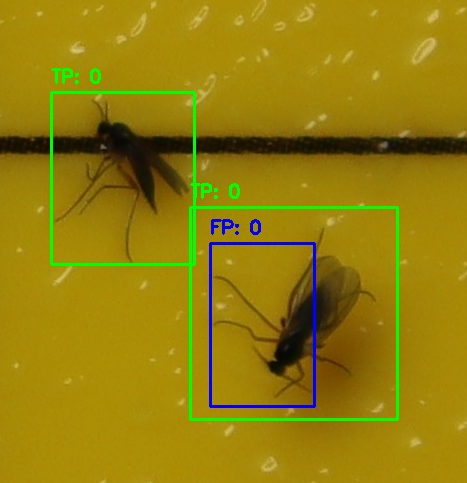
\includegraphics[width=\textwidth]{images/low_iou_nms_BRAIIM.png}
        \caption{Overlapping Bounding boxes not detected by NMS (fungus gnats)}
    \end{subfigure}
    \hfill
    \begin{subfigure}[b]{0.45\textwidth}
        \centering
        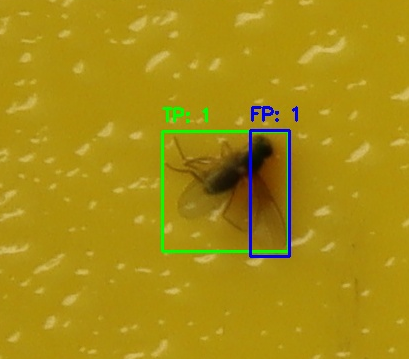
\includegraphics[width=\textwidth]{images/low_io_nms_LIRIBO.png}
        \caption{Overlapping Bounding boxes not detected by NMS (leaf miner fly)}
    \end{subfigure}
    
    % Second row
    \begin{subfigure}[b]{0.45\textwidth}
        \centering
        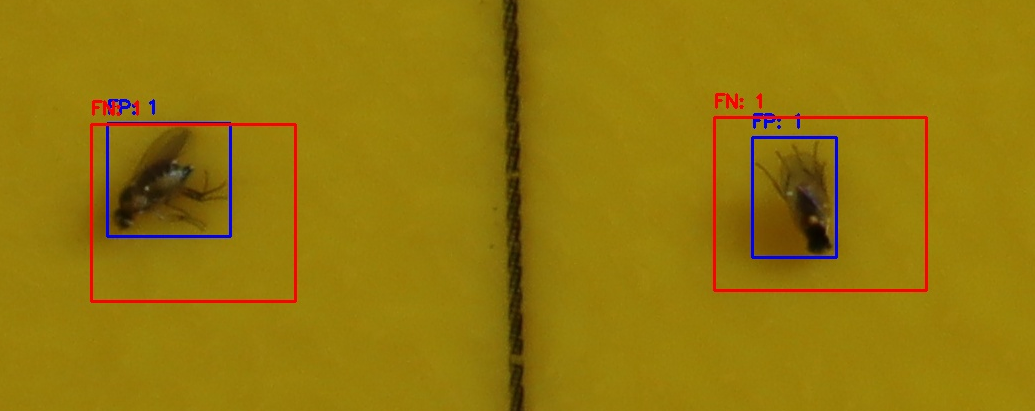
\includegraphics[width=\textwidth]{images/low_iou_LIRIBO.png}
        \caption{Bounding boxes counted as FP because of low IoU (leaf miner flies)}
    \end{subfigure}
    \hfill
    \begin{subfigure}[b]{0.45\textwidth}
        \centering
        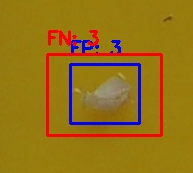
\includegraphics[width=\textwidth]{images/low_iou_TRIAVA.png}
        \caption{Bounding boxes counted as FP because of low IoU (whitefly)}
    \end{subfigure}
    
    \caption{Detection errors because of low IoU with small boxes. Green boxes are TP, blue boxes FP, red boxes FN}
    \label{fig:iou_problems}
\end{figure}

Visual inspection further revealed, that a proportion of the false positives are due to missing labels (see Figure~\ref{fig:false_positive_BRAIIMS}). Therefore for the best models the false positives in the test set are inspected visually and corrected precision metrics are calculated were necessary. 


\begin{figure}[H]  % 
    \centering
    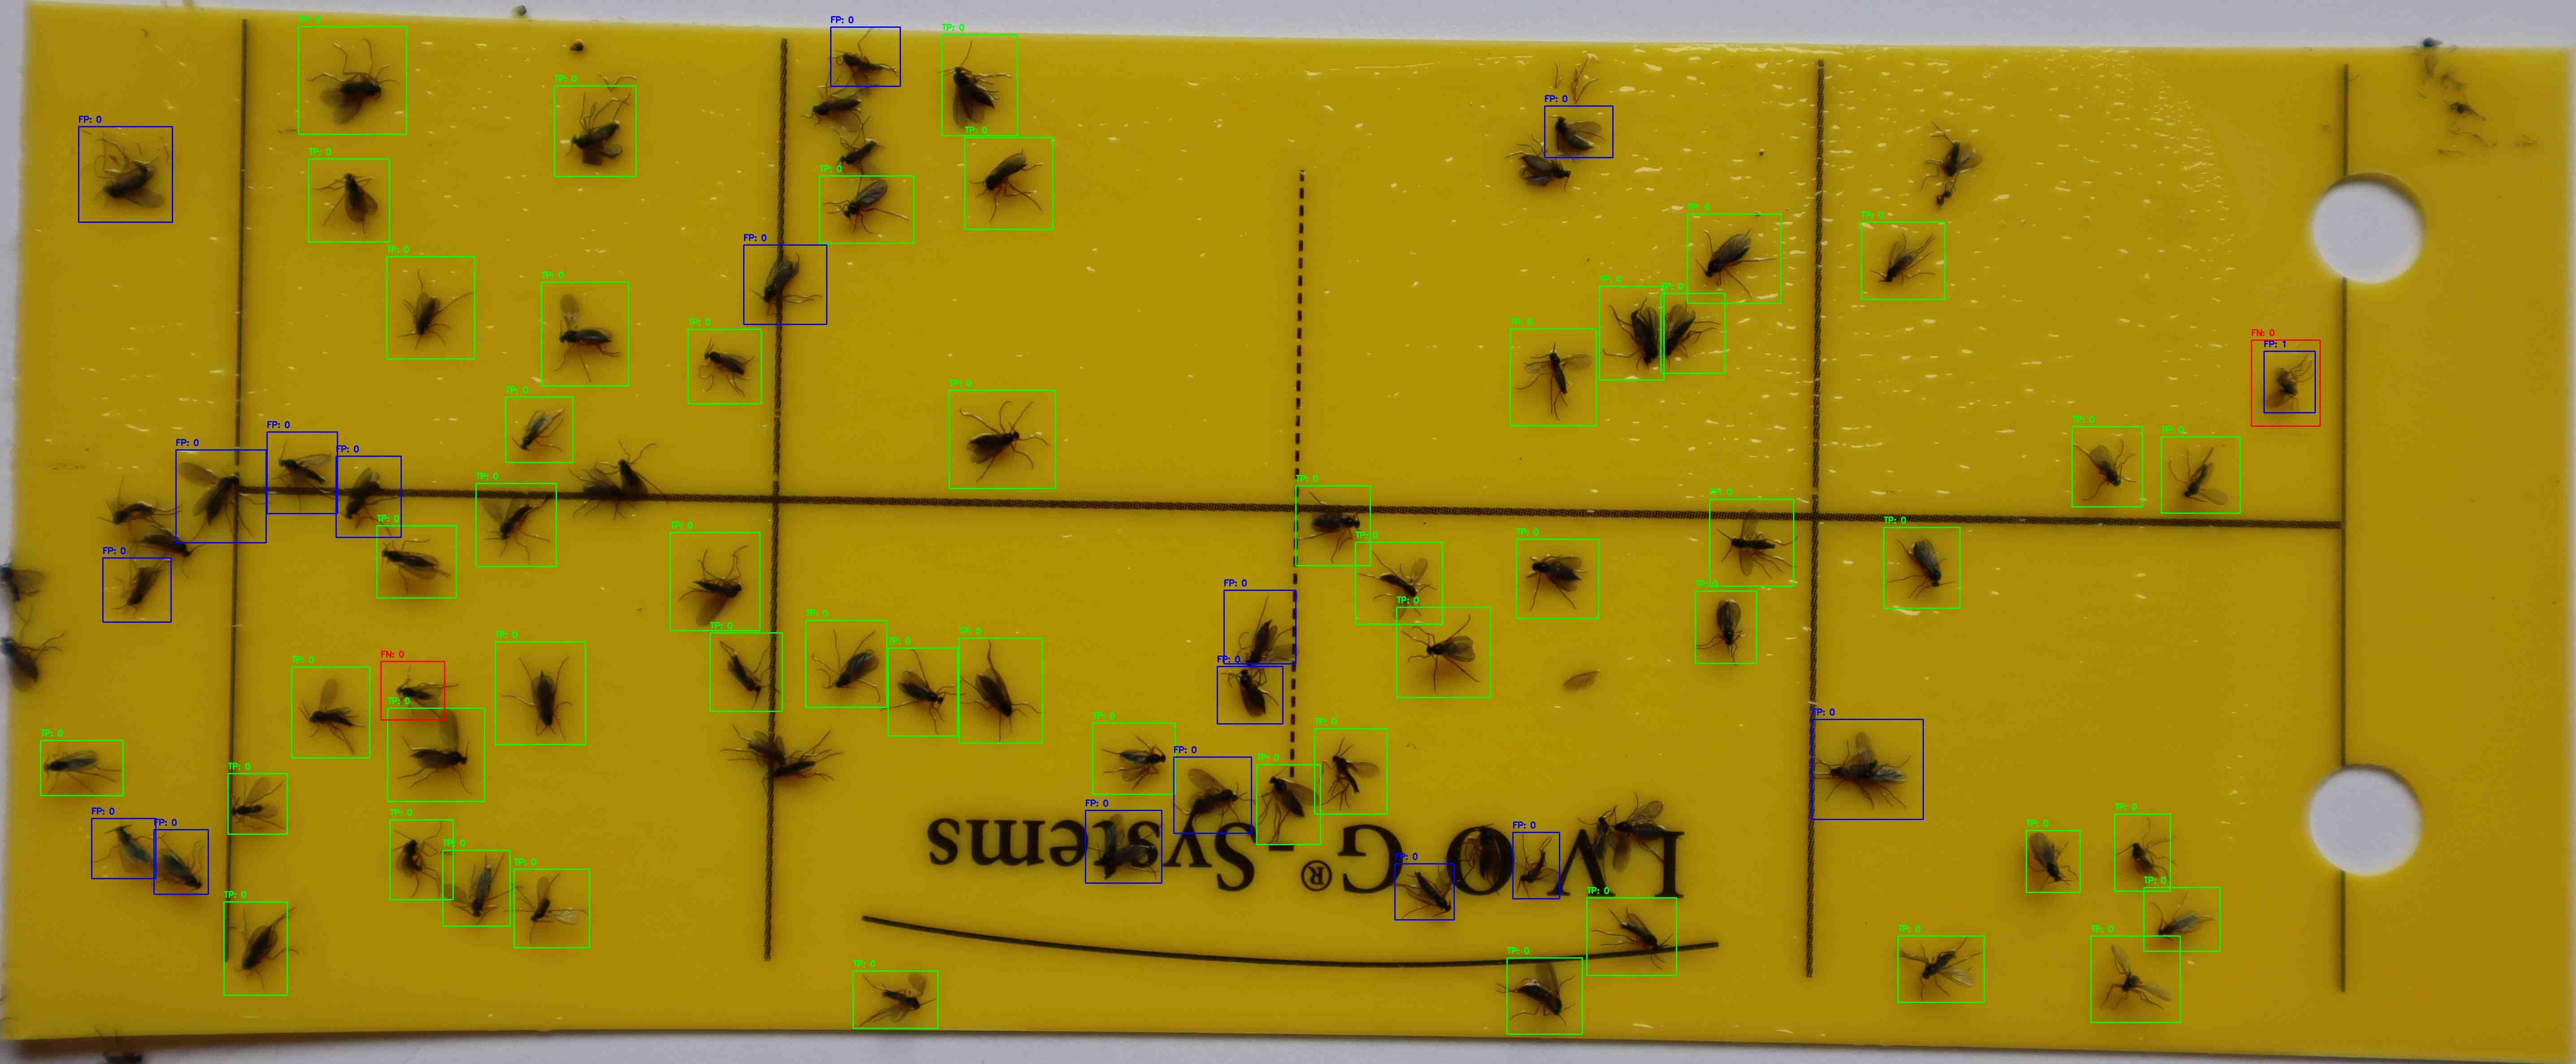
\includegraphics[width=1.0\textwidth]{images/false_positive_BRAIIM.jpg}  % Adjust width as needed
    \caption{False positive fungus gnats (blue boxes) are actually correct and only false due to missing labels. Green boxes are true positives, red false negatives.}
    \label{fig:false_positive_BRAIIMS}
\end{figure}

Metrics taken are per class as well as summarized precision, recall and F1 scores.






\subsection{Image processing}

%easy thresholds: size, color, orientation/shape
%edge density, texture
%selective search -> see papar in the original R_CNN [39]

%attention heads?
%will be low computation cost
%Clustering for improvement and for visualization may be implemented, as time allows.
%get thresholds

\subsection{Self-Training}

The SSL approach implemented in this work follows the self-training paradigm, originally introduced as ``pseudo-labeling'' by Lee (2013)~\cite{lee_pseudo-label_nodate}. In its simplest form, it entails training a model on a small amount of labeled data, use the model to predict on unlabeled data and then use the prediction as pseudo-labels to retrain the model. According to the comprehensive survey on the topic by Amini et al. (2025)~\cite{amini_self-training_2025}, self-training remains one of the most prevalent and effective strategies in semi-supervised learning, particularly in domains with partially labeled data. 

%The trained model is then used to generate predictions on both completely unlabeled and on the partially labeled data. The predictions generated by the model are filtered using a confidence threshold, and those above the threshold and not already labeled are considered pseudo-labels. These pseudo-labeled samples iteratively incorporated into subsequent rounds of training, gradually expanding and refining the training set. 
%YOLO8 or 9: has been proven to work for small objects (later transformer based models not so), is easier to hack, has lower training and inference costs - maybe test later versions.
%tiling?

%To mitigate the influence of potentially noisy pseudo-labels, the ratio between the labels generated by image processing and the pseudo-labeled data will be monitored and adjusted throughout training. Furthermore, a weighting scheme in the loss function will down-weight the contribution of pseudo-labeled data based on the iteration stage. The iterative process will be stopped when certain criteria are met. A key challenge of this approach is confirmation bias, where the model may reinforce false positives. To counteract this, several strategies will be considered and tested if necessary. These include augmentation-based regularization as proposed by Arazo et al. (2020)~\cite{arazo_pseudo-labeling_2020}, and more intricate teacher-student frameworks where one model generates pseudo-labels for another, as explored by Sohn et al. (2020)~\cite{sohn_simple_2020} and Pham et al. (2021)~\cite{pham_meta_2021}.

%The first test will be used to evaluate the stepwise improvement in the labels. The self-trained model will be evaluated using the second manually labeled test set.
%stopping criteria: These include observing a plateau in the number of new pseudo-labels generated per iteration or a stagnation in the distribution of pseudo-label confidence scores. 
%Additionally, a purely supervised baseline model will be trained on the labeled subset to quantify the performance improvements achieved through SSL.
%or do the baseline on the image processing labels?
%how many labels are need , how much data is needed
%self training domain shift amini 2025, https://www.sciencedirect.com/science/article/abs/pii/S1077314223000292
%%separate classification/object detection learning


\section{Results}

\subsection{Supervised training}
\label{sec:results_supervised}
In the training runs with all four insect pest classes included, the best balance of precision and recall was achieved in training run 7, which used 30\% background images and parameter set~1 with slight augmentations over 100 epochs (see Table~\ref{tab:thrips_included}, and compare Table~\ref{tab:paramters-supervised} and Table~\ref{tab:train_params} for settings). For testing, always the weights which gave the best results are taken, which are reported by YOLO and detected by the mAP@50:95 metric. Testing was performed with evaluation set~3, i.e., predictions with a confidence threshold of maximum F1 plus 0.1 and a stride of 420 for the sliding 640~$\times$~640 window. Longer training, as in training run~8, led to the best overall recall, but at the cost of reduced precision. The highest precision values were associated with the lowest recall values and were mostly obtained when applying stricter evaluation thresholds, as in evaluation sets~4 and~5. 

\begin{table}[h!]
\centering
\begin{tabular}{|c|c|c|c|c|}
\hline
train & eval & precision & recall & F1 \\
\hline
7 & 3 & 0.87 & 0.87 & \textbf{0.87} \\
8 & 3 & 0.85 & 0.88 & 0.87 \\
2 & 3 & 0.85 & \textbf{0.88} & 0.87 \\
3 & 3 & 0.86 & 0.87 & 0.87 \\
1 & 2 & 0.90 & 0.84 & 0.87 \\
1 & 1 & 0.88 & 0.84 & 0.86 \\
7 & 4 & 0.90 & 0.81 & 0.85 \\
6 & 3 & 0.89 & 0.81 & 0.85 \\
1 & 3 & 0.90 & 0.79 & 0.84 \\
3 & 4 & 0.90 & 0.79 & 0.84 \\
6 & 4 & 0.91 & 0.77 & 0.83 \\
7 & 5 & 0.91 & 0.76 & 0.83 \\
6 & 5 & \textbf{0.91} & 0.73 & 0.81 \\
\hline
\end{tabular}
\caption{Metrics with thrips included in training.}
\label{tab:thrips_included}
\end{table}

Table~\ref{tab:supervised_performance} summarizes the best results per class. For the F1 scores, leaf miner flies and whiteflies benefited slightly from training without thrips (runs~9 and~10), whereas thrips achieved their best value when empty images were included. Precision across all classes was maximized in the shorter training runs (100 epochs) combined with stricter confidence thresholds, with whiteflies in particular profiting from the stronger augmentations of parameter set~2 in run~3. Recall, in contrast, was highest in the longer training runs (8 and~10) with more lenient confidence thresholds; in this case, leaf miner flies profited from increased augmentations. 

\begin{landscape}
\begin{table}[h!]
\centering
\begin{tabular}{cccccccccccccc}
\hline
train & eval & Fun\_F1 & Leaf\_F1 & Whi\_F1 & Tr\_F1 & Fun\_P & Leaf\_P & Whi\_P & Tr\_P & Fun\_R & Leaf\_R & Whi\_R & Tr\_R \\
\hline
1 & 1 & 0.85 & 0.92 & 0.88 & \textbf{0.75} & 0.87 & 0.93 & 0.92 & 0.75 & 0.83 & 0.90 & 0.85 & 0.75 \\
1 & 2 & 0.88 & 0.92 & 0.89 & 0.72 & 0.89 & 0.93 & 0.93 & 0.79 & 0.87 & 0.91 & 0.86 & 0.67 \\
1 & 3 & 0.84 & 0.91 & 0.87 & 0.71 & 0.89 & 0.94 & 0.94 & 0.79 & 0.80 & 0.89 & 0.81 & 0.65 \\
2 & 3 & 0.88 & 0.93 & 0.90 & 0.73 & 0.85 & 0.92 & 0.92 & 0.68 & 0.90 & \textbf{0.94} & 0.89 & 0.79 \\
3 & 3 & 0.87 & 0.93 & 0.90 & 0.73 & 0.85 & 0.92 & 0.93 & 0.69 & 0.90 & 0.94 & 0.87 & 0.77 \\
3 & 4 & 0.87 & 0.93 & 0.85 & 0.67 & 0.88 & 0.93 & \textbf{0.95} & 0.77 & 0.86 & 0.92 & 0.78 & 0.59 \\
6 & 3 & 0.84 & 0.92 & 0.87 & 0.73 & 0.88 & 0.94 & 0.94 & 0.76 & 0.82 & 0.90 & 0.82 & 0.71 \\
6 & 4 & 0.87 & 0.93 & 0.85 & 0.63 & 0.89 & 0.94 & 0.95 & \textbf{0.82} & 0.84 & 0.92 & 0.76 & 0.52 \\
6 & 5 & 0.83 & 0.91 & 0.82 & 0.62 & \textbf{0.90} & 0.94 & 0.95 & 0.82 & 0.77 & 0.89 & 0.72 & 0.51 \\
7 & 3 & \textbf{0.88} & 0.93 & 0.90 & 0.74 & 0.86 & 0.93 & 0.93 & 0.72 & 0.89 & 0.93 & 0.88 & 0.76 \\
7 & 4 & 0.87 & 0.92 & 0.88 & 0.70 & 0.88 & 0.93 & 0.94 & 0.79 & 0.86 & 0.91 & 0.82 & 0.62 \\
7 & 5 & 0.83 & 0.91 & 0.85 & 0.69 & 0.89 & \textbf{0.94} & 0.95 & 0.80 & 0.78 & 0.87 & 0.77 & 0.60 \\
8 & 3 & 0.88 & 0.93 & 0.90 & 0.73 & 0.85 & 0.92 & 0.92 & 0.68 & \textbf{0.90} & 0.94 & 0.89 & \textbf{0.79} \\
9 & 3 & 0.88 & \textbf{0.94} & 0.89 & & 0.88 & 0.93 & 0.93 & & 0.88 & 0.94 & 0.85 & \\
10 & 3 & 0.88 & 0.93 & \textbf{0.91} & & 0.86 & 0.92 & 0.91 & & 0.89 & 0.93 & \textbf{0.92} & \\
\hline
\end{tabular}
\caption{Performance metrics for each train/eval combination, ordered by F1, precision, and recall values.}
\label{tab:supervised_performance}
\end{table}
\end{landscape}

The experiments were structured to first identify evaluation parameters that maximize precision on the dataset with all backgrounds included (see train~1, eval~1--3 in Table~\ref{tab:supervised_performance}). This showed that evaluation set~3 yielded the best per-class precision values. Reducing the proportion of background images in the training set shortens training time considerably. On a single GPU core {\color{red} Question@Martin: Which GPU?}, an epoch on the full training set takes ca. 18 minutes (100 epochs are approx. 30 hours) and on the training set with only 10\% images it takes ca. 7 min. (100 epochs are approx. 12 hours).

Therefore the subsequent runs aimed to reproduce or improve the results with reduced background-to-foreground ratios. Runs~2 and~3 used only 10\% background images with parameter sets~1 and~2, respectively. Runs~6 and~7 used 30\% background images and compared parameter set~2 (run~6) with set~1 (run~7), as well as the three evaluation settings~3--5, which led to the best overall results presented above. Run~8 tested the effect of longer training. Runs~9 and~10 explored shorter and longer training while excluding thrips images from the training set. Compared with the best results from run~7 (eval~3), the shorter run without thrips maintained precision and slightly improved recall for leaf miner flies. The longer run~10 again reduced per-class precision but achieved the best recall for whiteflies. Across all classes, run~10 slightly outperformed run~7. 

\begin{table}[h!]
\centering
\begin{tabular}{|c|c|c|c|c|c|}
\hline
train & eval & precision & recall & F1 & thrips included in training \\
\hline
10 & 3 & 0.90 & \textbf{0.91} & \textbf{0.91} & no \\
7 & 3 & \textbf{0.91} & 0.90 & 0.90 & yes \\
\hline
\end{tabular}
\caption{Metrics with thrips excluded from training.}
\label{tab:thrips_excluded}
\end{table}

Visual inspection of th false positives showed that for the fungus gnats a significant number of unlabeled images caused to false positives (see Figure~\ref{fig:false_positive_BRAIIMS} which in turns leads to a low precision. Therefore the common false positives predicted by the best model/evaluation pair train7/eval3 and train10/eval3 were selected, their confidence scores averaged and the predictions filtered for confidences higher than 0.6. This resulted in 156 predictions for the fungus gnats, 66 for the leaf miner flies and 91 for the whiteflies. As Figure~\ref{fig:fp_best_confidences} shows, the false positives for the last two pest classes are indeed of mixed quality. However, a visual inspection of the fungus gnat detections returned 116 correctly detected instances. {\color{red} Question@JKI: Is this correct? See images in Dropbox.} Recalculating the precision now returns precision 0.94 and 0.93 for the two best training results. With this correction, all classes but the thrips fulfill the required minimum precision and recall values (see Figure~\ref{fig:supervised_final_results} below).

\begin{figure}[h!]
    \centering
    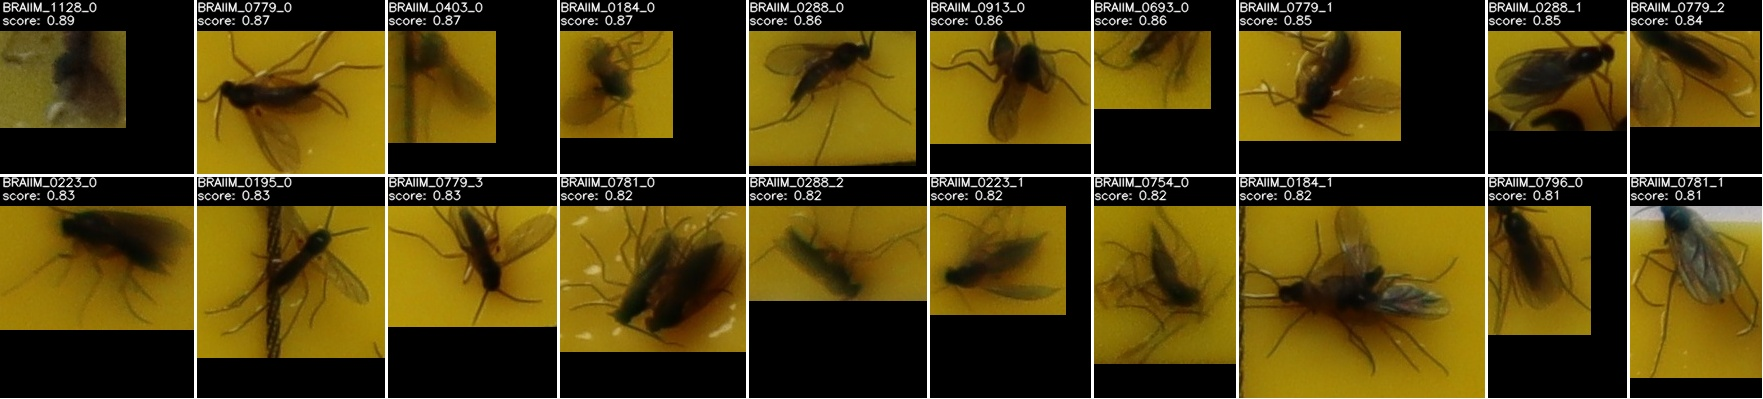
\includegraphics[width=\textwidth]{images/BRAIIM_fp_canvas_1.jpg} % first image
    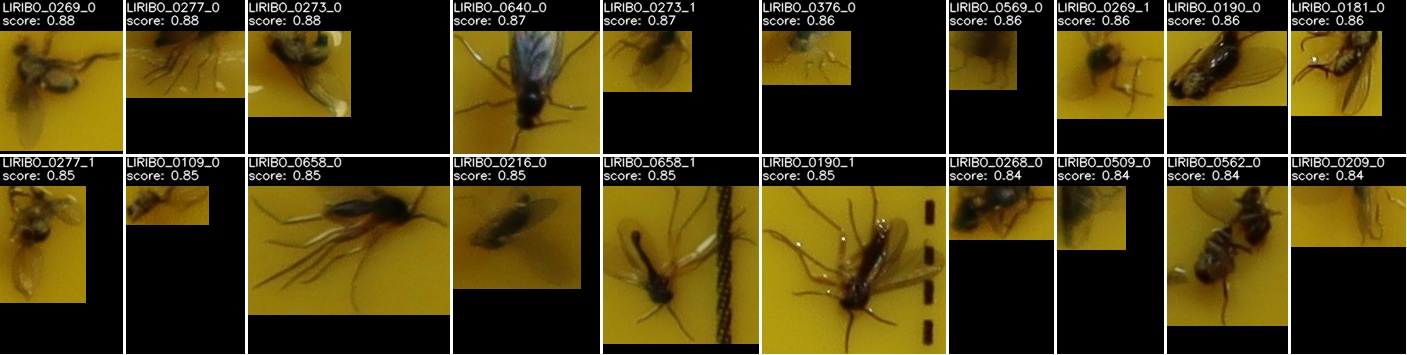
\includegraphics[width=\textwidth]{images/LIRIBO_fp_canvas_1.jpg} % second image
    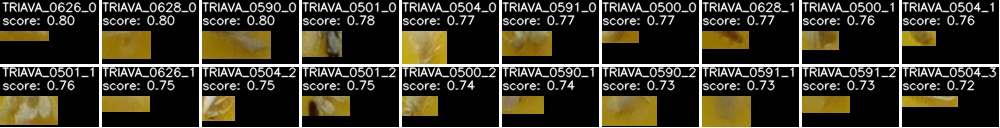
\includegraphics[width=\textwidth]{images/TRIAVA_fp_canvas_1.jpg} % third image
    \caption{False positive with maximum confidences for fungus gnats (BRAIIM), leaf miner flies (LIRIBO) and whiteflies (TRIAVA) (from top to bottom)}
    \label{fig:fp_best_confidences}
\end{figure}


\begin{figure}[H]
    \centering
    % Left image
    \begin{minipage}{0.48\textwidth}
        \centering
        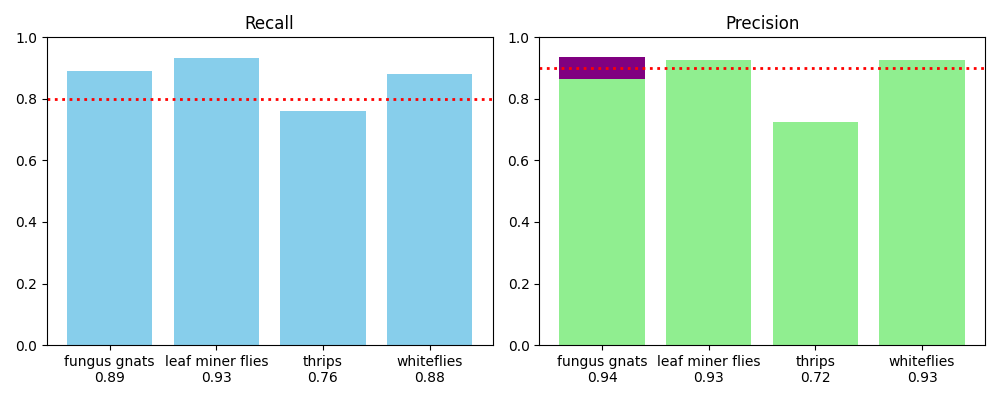
\includegraphics[width=\linewidth]{images/train7eval3.png}
        \caption{Results for training 7, evaluation set 3. Purple are the corrected labels.}
    \end{minipage}\hfill
    % Right image
    \begin{minipage}{0.48\textwidth}
        \centering
        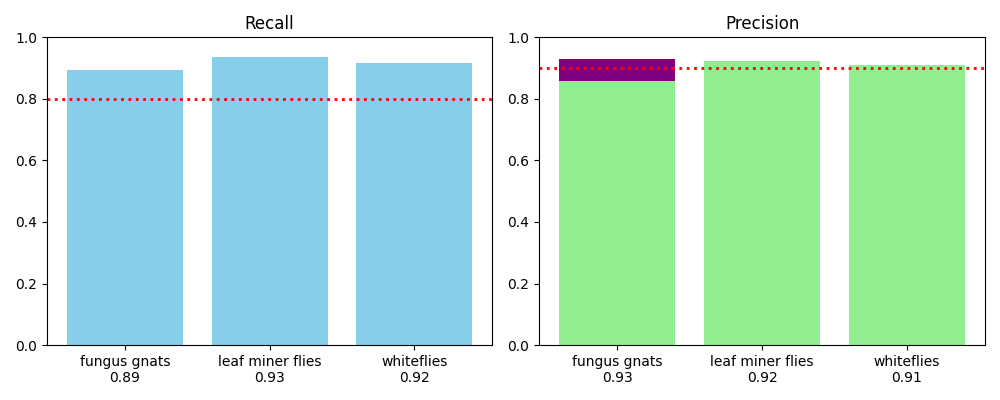
\includegraphics[width=\linewidth]{images/train10eval3.png}
        \caption{Results for training 10, evaluation set 3. Purple are the corrected labels.}
    \end{minipage}
    \caption{Results with corrected labels for fungus gnats false positives.}
    \label{fig:supervised_final_results}
\end{figure}

Comparing the validation metrics (Figure~\ref{fig:supervised_curves}) shows the improvements by reducing the background (upper to middle) and by omitting the thrips images (lower). Because the validation is done on tiles, metrics are not comparable to the metrics reported above, which were taken on full images. The loss curves in the two upper images still show underfitting, however, in the longer training (bottom) the balance between precision and recall degrades: Best mAP@50:05 is already in epoch 135 (which is chosen for above metrics) ({\color{red} ToDo: include the right mAP-metric in the graphs}), best recall is reported before, in epoch 124 but best precision is in epoch 162.

\begin{figure}[H]
    \centering
    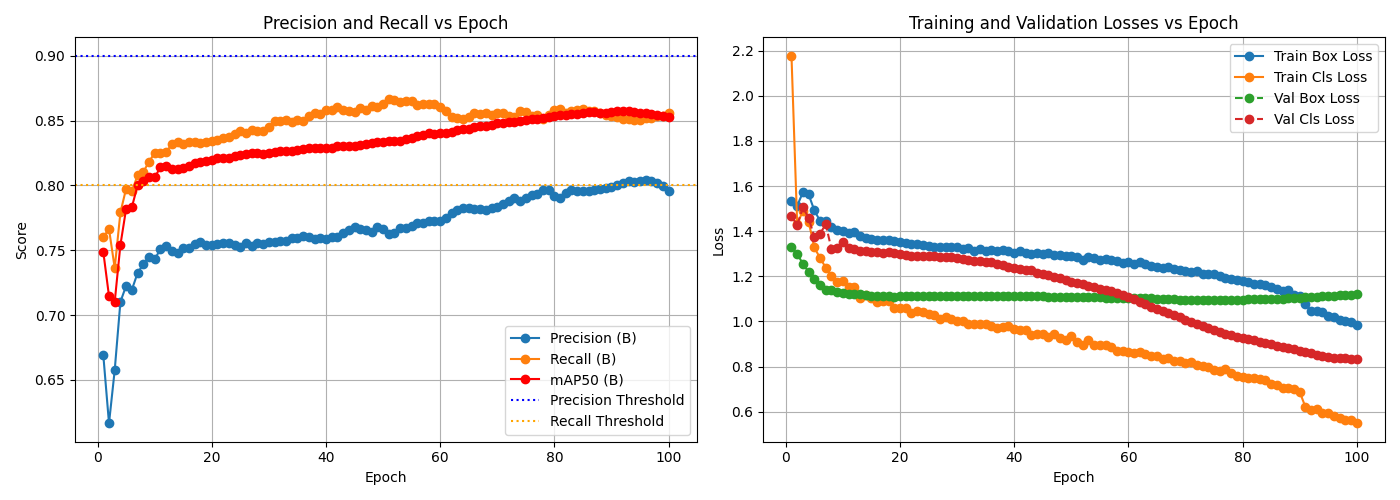
\includegraphics[width=\textwidth]{images/prec_recall_train.png} % first image
    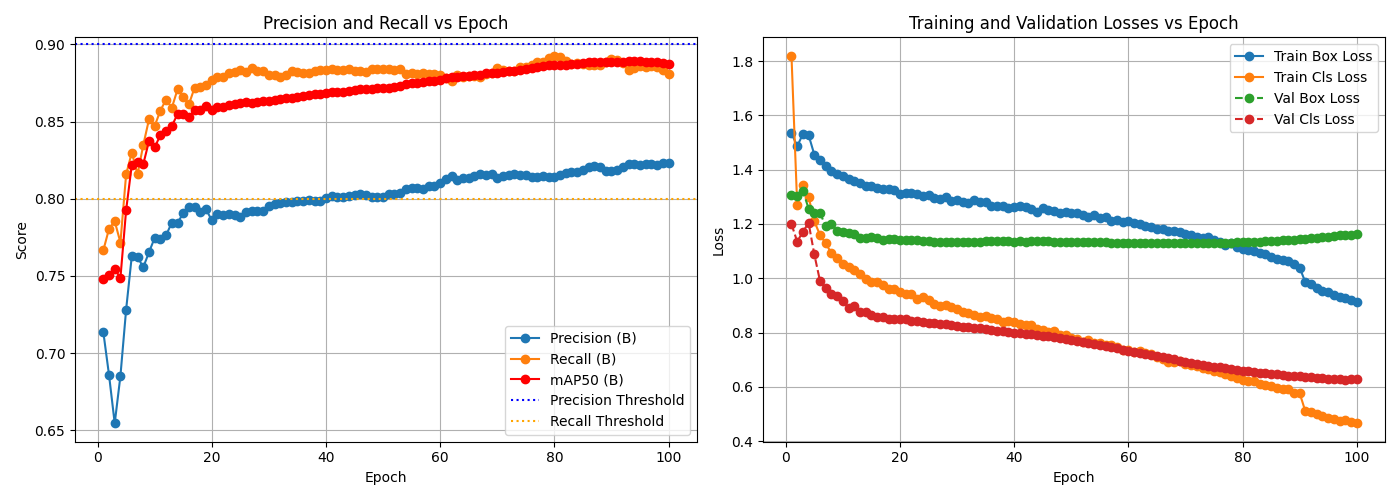
\includegraphics[width=\textwidth]{images/prec_recall_train7.png} % second image
    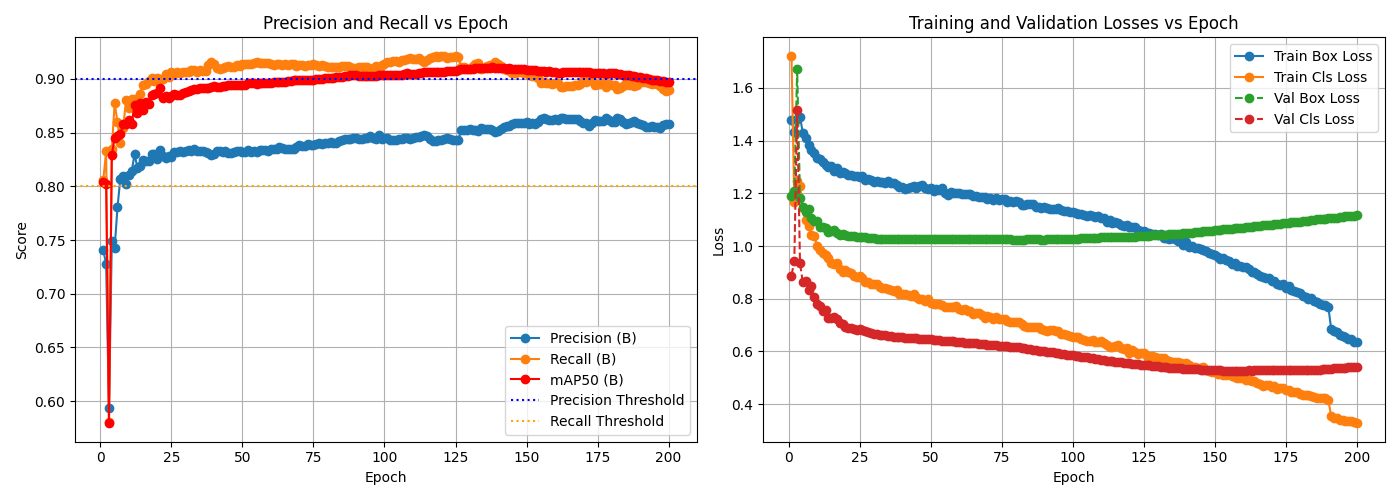
\includegraphics[width=\textwidth]{images/prec_recall_train10.png} % third image
    \caption{Validation metrics and loss curves for training run 1 (complete training set), 7 (background tiles reduced to 30\%) and 10 (without thrips, background images 47\%) (top to bottom)}
    \label{fig:supervised_curves}
\end{figure}


\section{Discussion}

results supervised: why the thrips are hard to detect? because male adults and larvae are so similar and the labels are ambiguous

Data in a later implementation will differ in at least two aspects. Most notably a domain shift has to be expected, as images taken in real use cases will likely be of much lower resolution. 
{\color{red} add picture of the checkpot? mention resolution of thrips, might be solvable by SSL, too
} Also, in the final usage, several pictures of the same YST are taken over the day. Because the individuals can interact with the glue and become partially hidden or change their appearance over time, this poses an additional problem to be addressed. If the difference between the individuals in the training data and those in the final data becomes too great, individuals might no longer be detected, and the population might be underestimated.
\section{Conclusion}



\section{References}
\printbibliography[heading=none]

\section{Glossary}


\begin{itemize}
    \item augmentation – Techniques that artificially increase dataset diversity by combining or altering images to improve model generalization.
    \item batches – Subsets of the dataset processed together during one iteration of training.
    \item class imbalance – When some classes appear much more frequently than others in the dataset, potentially biasing the model.
    \item COCO – A large-scale labeled image dataset commonly used for object detection and segmentation.
    \item color threshold based segmentation – A method to separate objects from the background based on color ranges.
    \item confidence – The probability assigned by a model to indicate how certain it is about a prediction.
    \item deep learning – Neural networks with multiple layers that learn features from data.
    \item domain shift – Differences between training and deployment data distributions that can reduce model performance.
    \item early stopping – A training strategy that stops training when the model performance on a validation set stops improving.
    \item epoch – Complete passes through the entire training dataset.
    \item F1-score – The harmonic mean of precision and recall, balancing false positives and false negatives.
    \item file checksums – Unique hash values used to verify file integrity; they are unambiguous identifiers for files.
    \item GPU – Graphics Processing Unit; used to accelerate large-scale computations for deep learning.
    \item grounding language-image model – Models that connect textual descriptions with images to detect or label objects.
    \item image processing – Processing images using algorithmic methods with manually designed features, as opposed to features learned automatically by deep learning models.
    \item IoU – Intersection over Union; a metric to measure the overlap between predicted and ground-truth bounding boxes.
    \item learning rate schedule – A strategy to adjust the optimizer’s learning rate during training to improve convergence.
    \item loss function – A function that quantifies the difference between predicted and true values, guiding the optimizer to adjust weights.  
    \item loss weights – Weights assigned to different components of a loss function to prioritize certain tasks or classes.
    \item mean average precision – A standard object detection metric averaging precision across classes and confidence thresholds.
    \item mixup (included in augmentation) – A specific data augmentation technique that blends two images and their labels.
    \item NMS – Non-Maximum Suppression; a method to remove redundant overlapping bounding boxes in detection.
    \item mosaic – A data augmentation technique that combines multiple images into one, helping the model learn context and improve generalization.  
    \item neural network – A computational model inspired by the brain, composed of interconnected nodes (neurons) that process data.
    \item optimizer – An algorithm that updates model parameters to minimize the loss function during training.
    \item padding – Adding extra pixels around images to make it divisible without remainder.  
    \item patience – Number of epochs to wait without improvement before applying early stopping.
    \item precision – The proportion of positive predictions that are correct.
    \item precision-recall curve – A graph showing the trade-off between precision and recall at different confidence thresholds.
    \item pretrained – Models previously trained on large datasets, used as a starting point for new tasks.
    \item pseudo-labels – Labels generated by a model for unlabeled data; used in self-training methods to improve learning.
    \item recall – The proportion of true positives correctly detected by the model.
    \item self-training – A semi-supervised method where a model trains on unlabeled data using its own predictions as labels.
    \item semi-supervised learning – Training with a combination of labeled and unlabeled data to reduce labeling effort.
    \item stride – The step size used when sliding over an image in a window or tiling an image. If the stride is equal to the size of the window, no overlaps are created.
    \item stochastic gradient descent – An optimizer that updates model parameters using gradients computed on batches of data.
    \item supervised training / learning – Training a model with input-output pairs where the correct output (label) is known.
    \item teacher-student – A semi-supervised training setup where a “teacher” model generates labels for a “student” model to learn from.
    \item validation set – A dataset used to monitor model performance during training; different from the test set, which is only used for final evaluation.  
    \item weights – The trainable parameters of a neural network that determine the influence of each input feature on the output.
    \item YOLO model – A real-time object detection neural network architecture designed for speed and accuracy.
\end{itemize}




\end{document}
